
\definecolor{c00007f}{RGB}{0,0,127}
\definecolor{cb2b2b2}{RGB}{178,178,178}
\definecolor{c7f0000}{RGB}{127,0,0}
\definecolor{cfff7cc}{RGB}{255,247,204}

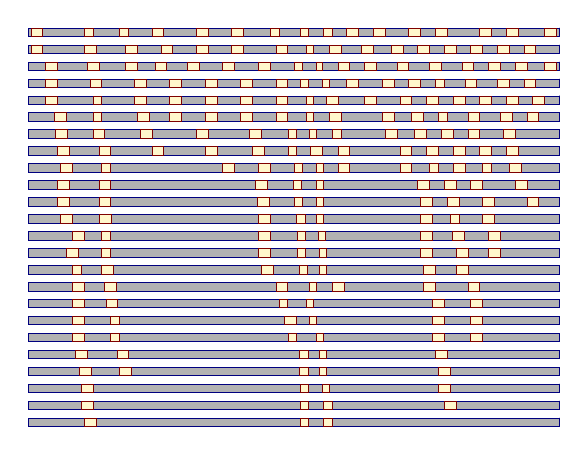
\begin{tikzpicture}[y=0.80pt, x=0.8pt,yscale=-1, inner sep=0pt, outer sep=0pt, scale=0.4,]
\begin{scope}% surface39
  % path249
  \path[draw=c00007f,fill=cb2b2b2,line join=miter,line cap=butt,miter
    limit=10.00,nonzero rule,line width=0.153pt] (0.0000,0.0000) --
    (600.0000,0.0000) -- (600.0000,9.5742) -- (0.0000,9.5742) --
    cycle(0.0000,0.0000);

  % path251
  \path[draw=c00007f,fill=cb2b2b2,line join=miter,line cap=butt,miter
    limit=10.00,nonzero rule,line width=0.153pt] (600.0000,0.0000) --
    (600.0000,9.5742) -- cycle(600.0000,0.0000);

  % path253
  \path[draw=c00007f,fill=cb2b2b2,line join=miter,line cap=butt,miter
    limit=10.00,nonzero rule,line width=0.153pt] (0.0000,19.1484) --
    (600.0000,19.1484) -- (600.0000,28.7227) -- (0.0000,28.7227) --
    cycle(0.0000,19.1484);

  % path255
  \path[draw=c00007f,fill=cb2b2b2,line join=miter,line cap=butt,miter
    limit=10.00,nonzero rule,line width=0.153pt] (600.0000,19.1484) --
    (600.0000,28.7227) -- cycle(600.0000,19.1484);

  % path257
  \path[draw=c00007f,fill=cb2b2b2,line join=miter,line cap=butt,miter
    limit=10.00,nonzero rule,line width=0.153pt] (0.0000,38.2969) --
    (600.0000,38.2969) -- (600.0000,47.8711) -- (0.0000,47.8711) --
    cycle(0.0000,38.2969);

  % path259
  \path[draw=c00007f,fill=cb2b2b2,line join=miter,line cap=butt,miter
    limit=10.00,nonzero rule,line width=0.153pt] (600.0000,38.2969) --
    (600.0000,47.8711) -- cycle(600.0000,38.2969);

  % path261
  \path[draw=c00007f,fill=cb2b2b2,line join=miter,line cap=butt,miter
    limit=10.00,nonzero rule,line width=0.153pt] (0.0000,57.4453) --
    (600.0000,57.4453) -- (600.0000,67.0195) -- (0.0000,67.0195) --
    cycle(0.0000,57.4453);

  % path263
  \path[draw=c00007f,fill=cb2b2b2,line join=miter,line cap=butt,miter
    limit=10.00,nonzero rule,line width=0.153pt] (600.0000,57.4453) --
    (600.0000,67.0195) -- cycle(600.0000,57.4453);

  % path265
  \path[draw=c00007f,fill=cb2b2b2,line join=miter,line cap=butt,miter
    limit=10.00,nonzero rule,line width=0.153pt] (0.0000,76.5977) --
    (600.0000,76.5977) -- (600.0000,86.1719) -- (0.0000,86.1719) --
    cycle(0.0000,76.5977);

  % path267
  \path[draw=c00007f,fill=cb2b2b2,line join=miter,line cap=butt,miter
    limit=10.00,nonzero rule,line width=0.153pt] (600.0000,76.5977) --
    (600.0000,86.1719) -- cycle(600.0000,76.5977);

  % path269
  \path[draw=c00007f,fill=cb2b2b2,line join=miter,line cap=butt,miter
    limit=10.00,nonzero rule,line width=0.153pt] (0.0000,95.7461) --
    (600.0000,95.7461) -- (600.0000,105.3203) -- (0.0000,105.3203) --
    cycle(0.0000,95.7461);

  % path271
  \path[draw=c00007f,fill=cb2b2b2,line join=miter,line cap=butt,miter
    limit=10.00,nonzero rule,line width=0.153pt] (600.0000,95.7461) --
    (600.0000,105.3203) -- cycle(600.0000,95.7461);

  % path273
  \path[draw=c00007f,fill=cb2b2b2,line join=miter,line cap=butt,miter
    limit=10.00,nonzero rule,line width=0.153pt] (0.0000,114.8945) --
    (600.0000,114.8945) -- (600.0000,124.4688) -- (0.0000,124.4688) --
    cycle(0.0000,114.8945);

  % path275
  \path[draw=c00007f,fill=cb2b2b2,line join=miter,line cap=butt,miter
    limit=10.00,nonzero rule,line width=0.153pt] (600.0000,114.8945) --
    (600.0000,124.4688) -- cycle(600.0000,114.8945);

  % path277
  \path[draw=c00007f,fill=cb2b2b2,line join=miter,line cap=butt,miter
    limit=10.00,nonzero rule,line width=0.153pt] (0.0000,134.0430) --
    (600.0000,134.0430) -- (600.0000,143.6172) -- (0.0000,143.6172) --
    cycle(0.0000,134.0430);

  % path279
  \path[draw=c00007f,fill=cb2b2b2,line join=miter,line cap=butt,miter
    limit=10.00,nonzero rule,line width=0.153pt] (600.0000,134.0430) --
    (600.0000,143.6172) -- cycle(600.0000,134.0430);

  % path281
  \path[draw=c00007f,fill=cb2b2b2,line join=miter,line cap=butt,miter
    limit=10.00,nonzero rule,line width=0.153pt] (0.0000,153.1914) --
    (600.0000,153.1914) -- (600.0000,162.7656) -- (0.0000,162.7656) --
    cycle(0.0000,153.1914);

  % path283
  \path[draw=c00007f,fill=cb2b2b2,line join=miter,line cap=butt,miter
    limit=10.00,nonzero rule,line width=0.153pt] (600.0000,153.1914) --
    (600.0000,162.7656) -- cycle(600.0000,153.1914);

  % path285
  \path[draw=c00007f,fill=cb2b2b2,line join=miter,line cap=butt,miter
    limit=10.00,nonzero rule,line width=0.153pt] (0.0000,172.3398) --
    (600.0000,172.3398) -- (600.0000,181.9141) -- (0.0000,181.9141) --
    cycle(0.0000,172.3398);

  % path287
  \path[draw=c00007f,fill=cb2b2b2,line join=miter,line cap=butt,miter
    limit=10.00,nonzero rule,line width=0.153pt] (600.0000,172.3398) --
    (600.0000,181.9141) -- cycle(600.0000,172.3398);

  % path289
  \path[draw=c00007f,fill=cb2b2b2,line join=miter,line cap=butt,miter
    limit=10.00,nonzero rule,line width=0.153pt] (0.0000,191.4883) --
    (600.0000,191.4883) -- (600.0000,201.0625) -- (0.0000,201.0625) --
    cycle(0.0000,191.4883);

  % path291
  \path[draw=c00007f,fill=cb2b2b2,line join=miter,line cap=butt,miter
    limit=10.00,nonzero rule,line width=0.153pt] (600.0000,191.4883) --
    (600.0000,201.0625) -- cycle(600.0000,191.4883);

  % path293
  \path[draw=c00007f,fill=cb2b2b2,line join=miter,line cap=butt,miter
    limit=10.00,nonzero rule,line width=0.153pt] (0.0000,210.6367) --
    (600.0000,210.6367) -- (600.0000,220.2109) -- (0.0000,220.2109) --
    cycle(0.0000,210.6367);

  % path295
  \path[draw=c00007f,fill=cb2b2b2,line join=miter,line cap=butt,miter
    limit=10.00,nonzero rule,line width=0.153pt] (600.0000,210.6367) --
    (600.0000,220.2109) -- cycle(600.0000,210.6367);

  % path297
  \path[draw=c00007f,fill=cb2b2b2,line join=miter,line cap=butt,miter
    limit=10.00,nonzero rule,line width=0.153pt] (0.0000,229.7891) --
    (600.0000,229.7891) -- (600.0000,239.3633) -- (0.0000,239.3633) --
    cycle(0.0000,229.7891);

  % path299
  \path[draw=c00007f,fill=cb2b2b2,line join=miter,line cap=butt,miter
    limit=10.00,nonzero rule,line width=0.153pt] (600.0000,229.7891) --
    (600.0000,239.3633) -- cycle(600.0000,229.7891);

  % path301
  \path[draw=c00007f,fill=cb2b2b2,line join=miter,line cap=butt,miter
    limit=10.00,nonzero rule,line width=0.153pt] (0.0000,248.9375) --
    (600.0000,248.9375) -- (600.0000,258.5117) -- (0.0000,258.5117) --
    cycle(0.0000,248.9375);

  % path303
  \path[draw=c00007f,fill=cb2b2b2,line join=miter,line cap=butt,miter
    limit=10.00,nonzero rule,line width=0.153pt] (600.0000,248.9375) --
    (600.0000,258.5117) -- cycle(600.0000,248.9375);

  % path305
  \path[draw=c00007f,fill=cb2b2b2,line join=miter,line cap=butt,miter
    limit=10.00,nonzero rule,line width=0.153pt] (0.0000,268.0859) --
    (600.0000,268.0859) -- (600.0000,277.6602) -- (0.0000,277.6602) --
    cycle(0.0000,268.0859);

  % path307
  \path[draw=c00007f,fill=cb2b2b2,line join=miter,line cap=butt,miter
    limit=10.00,nonzero rule,line width=0.153pt] (600.0000,268.0859) --
    (600.0000,277.6602) -- cycle(600.0000,268.0859);

  % path309
  \path[draw=c00007f,fill=cb2b2b2,line join=miter,line cap=butt,miter
    limit=10.00,nonzero rule,line width=0.153pt] (0.0000,287.2344) --
    (600.0000,287.2344) -- (600.0000,296.8086) -- (0.0000,296.8086) --
    cycle(0.0000,287.2344);

  % path311
  \path[draw=c00007f,fill=cb2b2b2,line join=miter,line cap=butt,miter
    limit=10.00,nonzero rule,line width=0.153pt] (600.0000,287.2344) --
    (600.0000,296.8086) -- cycle(600.0000,287.2344);

  % path313
  \path[draw=c00007f,fill=cb2b2b2,line join=miter,line cap=butt,miter
    limit=10.00,nonzero rule,line width=0.153pt] (0.0000,306.3828) --
    (600.0000,306.3828) -- (600.0000,315.9570) -- (0.0000,315.9570) --
    cycle(0.0000,306.3828);

  % path315
  \path[draw=c00007f,fill=cb2b2b2,line join=miter,line cap=butt,miter
    limit=10.00,nonzero rule,line width=0.153pt] (600.0000,306.3828) --
    (600.0000,315.9570) -- cycle(600.0000,306.3828);

  % path317
  \path[draw=c00007f,fill=cb2b2b2,line join=miter,line cap=butt,miter
    limit=10.00,nonzero rule,line width=0.153pt] (0.0000,325.5313) --
    (600.0000,325.5313) -- (600.0000,335.1055) -- (0.0000,335.1055) --
    cycle(0.0000,325.5313);

  % path319
  \path[draw=c00007f,fill=cb2b2b2,line join=miter,line cap=butt,miter
    limit=10.00,nonzero rule,line width=0.153pt] (600.0000,325.5313) --
    (600.0000,335.1055) -- cycle(600.0000,325.5313);

  % path321
  \path[draw=c00007f,fill=cb2b2b2,line join=miter,line cap=butt,miter
    limit=10.00,nonzero rule,line width=0.153pt] (0.0000,344.6797) --
    (600.0000,344.6797) -- (600.0000,354.2539) -- (0.0000,354.2539) --
    cycle(0.0000,344.6797);

  % path323
  \path[draw=c00007f,fill=cb2b2b2,line join=miter,line cap=butt,miter
    limit=10.00,nonzero rule,line width=0.153pt] (600.0000,344.6797) --
    (600.0000,354.2539) -- cycle(600.0000,344.6797);

  % path325
  \path[draw=c00007f,fill=cb2b2b2,line join=miter,line cap=butt,miter
    limit=10.00,nonzero rule,line width=0.153pt] (0.0000,363.8281) --
    (600.0000,363.8281) -- (600.0000,373.4023) -- (0.0000,373.4023) --
    cycle(0.0000,363.8281);

  % path327
  \path[draw=c00007f,fill=cb2b2b2,line join=miter,line cap=butt,miter
    limit=10.00,nonzero rule,line width=0.153pt] (600.0000,363.8281) --
    (600.0000,373.4023) -- cycle(600.0000,363.8281);

  % path329
  \path[draw=c00007f,fill=cb2b2b2,line join=miter,line cap=butt,miter
    limit=10.00,nonzero rule,line width=0.153pt] (0.0000,382.9805) --
    (600.0000,382.9805) -- (600.0000,392.5547) -- (0.0000,392.5547) --
    cycle(0.0000,382.9805);

  % path331
  \path[draw=c00007f,fill=cb2b2b2,line join=miter,line cap=butt,miter
    limit=10.00,nonzero rule,line width=0.153pt] (600.0000,382.9805) --
    (600.0000,392.5547) -- cycle(600.0000,382.9805);

  % path333
  \path[draw=c00007f,fill=cb2b2b2,line join=miter,line cap=butt,miter
    limit=10.00,nonzero rule,line width=0.153pt] (0.0000,402.1289) --
    (600.0000,402.1289) -- (600.0000,411.7031) -- (0.0000,411.7031) --
    cycle(0.0000,402.1289);

  % path335
  \path[draw=c00007f,fill=cb2b2b2,line join=miter,line cap=butt,miter
    limit=10.00,nonzero rule,line width=0.153pt] (600.0000,402.1289) --
    (600.0000,411.7031) -- cycle(600.0000,402.1289);

  % path337
  \path[draw=c00007f,fill=cb2b2b2,line join=miter,line cap=butt,miter
    limit=10.00,nonzero rule,line width=0.153pt] (0.0000,421.2773) --
    (600.0000,421.2773) -- (600.0000,430.8516) -- (0.0000,430.8516) --
    cycle(0.0000,421.2773);

  % path339
  \path[draw=c00007f,fill=cb2b2b2,line join=miter,line cap=butt,miter
    limit=10.00,nonzero rule,line width=0.153pt] (600.0000,421.2773) --
    (600.0000,430.8516) -- cycle(600.0000,421.2773);

  % path341
  \path[draw=c00007f,fill=cb2b2b2,line join=miter,line cap=butt,miter
    limit=10.00,nonzero rule,line width=0.153pt] (0.0000,440.4258) --
    (600.0000,440.4258) -- (600.0000,450.0000) -- (0.0000,450.0000) --
    cycle(0.0000,440.4258);

  % path343
  \path[draw=c00007f,fill=cb2b2b2,line join=miter,line cap=butt,miter
    limit=10.00,nonzero rule,line width=0.153pt] (600.0000,440.4258) --
    (600.0000,450.0000) -- cycle(600.0000,440.4258);

  % path345
  \path[draw=c7f0000,fill=cfff7cc,line join=miter,line cap=butt,miter
    limit=10.00,nonzero rule,line width=0.153pt] (3.3320,0.0000) --
    (16.6641,0.0000) -- (16.6641,9.5742) -- (3.3320,9.5742) --
    cycle(3.3320,0.0000);

  \begin{scope}[fill=black]% g347
    \begin{scope}[shift={(5.5,4.789062)}]% use349
    \end{scope}
    \begin{scope}[shift={(10.5,4.789062)}]% use351
    \end{scope}
  \end{scope}
  % path353
  \path[draw=c7f0000,fill=cfff7cc,line join=miter,line cap=butt,miter
    limit=10.00,nonzero rule,line width=0.153pt] (3.3320,19.1484) --
    (16.6641,19.1484) -- (16.6641,28.7227) -- (3.3320,28.7227) --
    cycle(3.3320,19.1484);

  \begin{scope}[fill=black]% g355
    \begin{scope}[shift={(3.5,23.9375)}]% use357
    \end{scope}
    \begin{scope}[shift={(8.5,23.9375)}]% use359
    \end{scope}
    \begin{scope}[shift={(13.5,23.9375)}]% use361
    \end{scope}
  \end{scope}
  % path363
  \path[draw=c7f0000,fill=cfff7cc,line join=miter,line cap=butt,miter
    limit=10.00,nonzero rule,line width=0.153pt] (20.0000,38.2969) --
    (33.3320,38.2969) -- (33.3320,47.8711) -- (20.0000,47.8711) --
    cycle(20.0000,38.2969);

  \begin{scope}[fill=black]% g365
    \begin{scope}[shift={(20.167969,43.085938)}]% use367
    \end{scope}
    \begin{scope}[shift={(25.167969,43.085938)}]% use369
    \end{scope}
    \begin{scope}[shift={(30.167969,43.085938)}]% use371
    \end{scope}
  \end{scope}
  % path373
  \path[draw=c7f0000,fill=cfff7cc,line join=miter,line cap=butt,miter
    limit=10.00,nonzero rule,line width=0.153pt] (20.0000,57.4453) --
    (33.3320,57.4453) -- (33.3320,67.0195) -- (20.0000,67.0195) --
    cycle(20.0000,57.4453);

  \begin{scope}[fill=black]% g375
    \begin{scope}[shift={(19.667969,62.234375)}]% use377
    \end{scope}
    \begin{scope}[shift={(24.667969,62.234375)}]% use379
    \end{scope}
    \begin{scope}[shift={(29.667969,62.234375)}]% use381
    \end{scope}
  \end{scope}
  % path383
  \path[draw=c7f0000,fill=cfff7cc,line join=miter,line cap=butt,miter
    limit=10.00,nonzero rule,line width=0.153pt] (20.0000,76.5977) --
    (33.3320,76.5977) -- (33.3320,86.1719) -- (20.0000,86.1719) --
    cycle(20.0000,76.5977);

  \begin{scope}[fill=black]% g385
    \begin{scope}[shift={(22.167969,81.382812)}]% use387
    \end{scope}
    \begin{scope}[shift={(27.167969,81.382812)}]% use389
    \end{scope}
  \end{scope}
  % path391
  \path[draw=c7f0000,fill=cfff7cc,line join=miter,line cap=butt,miter
    limit=10.00,nonzero rule,line width=0.153pt] (30.0000,95.7461) --
    (43.3320,95.7461) -- (43.3320,105.3203) -- (30.0000,105.3203) --
    cycle(30.0000,95.7461);

  \begin{scope}[fill=black]% g393
    \begin{scope}[shift={(32.667969,100.53125)}]% use395
    \end{scope}
    \begin{scope}[shift={(37.667969,100.53125)}]% use397
    \end{scope}
  \end{scope}
  % path399
  \path[draw=c7f0000,fill=cfff7cc,line join=miter,line cap=butt,miter
    limit=10.00,nonzero rule,line width=0.153pt] (31.3320,114.8945) --
    (44.6641,114.8945) -- (44.6641,124.4688) -- (31.3320,124.4688) --
    cycle(31.3320,114.8945);

  \begin{scope}[fill=black]% g401
    \begin{scope}[shift={(31.5,119.679688)}]% use403
    \end{scope}
    \begin{scope}[shift={(36.5,119.679688)}]% use405
    \end{scope}
    \begin{scope}[shift={(41.5,119.679688)}]% use407
    \end{scope}
  \end{scope}
  % path409
  \path[draw=c7f0000,fill=cfff7cc,line join=miter,line cap=butt,miter
    limit=10.00,nonzero rule,line width=0.153pt] (33.3320,134.0430) --
    (46.6641,134.0430) -- (46.6641,143.6172) -- (33.3320,143.6172) --
    cycle(33.3320,134.0430);

  \begin{scope}[fill=black]% g411
    \begin{scope}[shift={(33.0,138.828125)}]% use413
    \end{scope}
    \begin{scope}[shift={(38.0,138.828125)}]% use415
    \end{scope}
    \begin{scope}[shift={(43.0,138.828125)}]% use417
    \end{scope}
  \end{scope}
  % path419
  \path[draw=c7f0000,fill=cfff7cc,line join=miter,line cap=butt,miter
    limit=10.00,nonzero rule,line width=0.153pt] (33.3320,191.4883) --
    (46.6641,191.4883) -- (46.6641,201.0625) -- (33.3320,201.0625) --
    cycle(33.3320,191.4883);

  \begin{scope}[fill=black]% g421
    \begin{scope}[shift={(33.0,196.277344)}]% use423
    \end{scope}
    \begin{scope}[shift={(38.0,196.277344)}]% use425
    \end{scope}
    \begin{scope}[shift={(43.0,196.277344)}]% use427
    \end{scope}
  \end{scope}
  % path429
  \path[draw=c7f0000,fill=cfff7cc,line join=miter,line cap=butt,miter
    limit=10.00,nonzero rule,line width=0.153pt] (33.3320,172.3398) --
    (46.6641,172.3398) -- (46.6641,181.9141) -- (33.3320,181.9141) --
    cycle(33.3320,172.3398);

  \begin{scope}[fill=black]% g431
    \begin{scope}[shift={(36.0,177.128906)}]% use433
    \end{scope}
    \begin{scope}[shift={(41.0,177.128906)}]% use435
    \end{scope}
  \end{scope}
  % path437
  \path[draw=c7f0000,fill=cfff7cc,line join=miter,line cap=butt,miter
    limit=10.00,nonzero rule,line width=0.153pt] (36.6680,153.1914) --
    (50.0000,153.1914) -- (50.0000,162.7656) -- (36.6680,162.7656) --
    cycle(36.6680,153.1914);

  \begin{scope}[fill=black]% g439
    \begin{scope}[shift={(36.832031,157.980469)}]% use441
    \end{scope}
    \begin{scope}[shift={(41.832031,157.980469)}]% use443
    \end{scope}
    \begin{scope}[shift={(46.832031,157.980469)}]% use445
    \end{scope}
  \end{scope}
  % path447
  \path[draw=c7f0000,fill=cfff7cc,line join=miter,line cap=butt,miter
    limit=10.00,nonzero rule,line width=0.153pt] (36.6680,210.6367) --
    (50.0000,210.6367) -- (50.0000,220.2109) -- (36.6680,220.2109) --
    cycle(36.6680,210.6367);

  \begin{scope}[fill=black]% g449
    \begin{scope}[shift={(36.832031,215.425781)}]% use451
    \end{scope}
    \begin{scope}[shift={(41.832031,215.425781)}]% use453
    \end{scope}
    \begin{scope}[shift={(46.832031,215.425781)}]% use455
    \end{scope}
  \end{scope}
  % path457
  \path[draw=c7f0000,fill=cfff7cc,line join=miter,line cap=butt,miter
    limit=10.00,nonzero rule,line width=0.153pt] (43.3320,248.9375) --
    (56.6641,248.9375) -- (56.6641,258.5117) -- (43.3320,258.5117) --
    cycle(43.3320,248.9375);

  \begin{scope}[fill=black]% g459
    \begin{scope}[shift={(43.0,253.722656)}]% use461
    \end{scope}
    \begin{scope}[shift={(48.0,253.722656)}]% use463
    \end{scope}
    \begin{scope}[shift={(53.0,253.722656)}]% use465
    \end{scope}
  \end{scope}
  % path467
  \path[draw=c7f0000,fill=cfff7cc,line join=miter,line cap=butt,miter
    limit=10.00,nonzero rule,line width=0.153pt] (50.0000,268.0859) --
    (60.0000,268.0859) -- (60.0000,277.6602) -- (50.0000,277.6602) --
    cycle(50.0000,268.0859);

  \begin{scope}[fill=black]% g469
    \begin{scope}[shift={(48.5,272.871094)}]% use471
    \end{scope}
    \begin{scope}[shift={(53.5,272.871094)}]% use473
    \end{scope}
    \begin{scope}[shift={(58.5,272.871094)}]% use475
    \end{scope}
  \end{scope}
  % path477
  \path[draw=c7f0000,fill=cfff7cc,line join=miter,line cap=butt,miter
    limit=10.00,nonzero rule,line width=0.153pt] (50.0000,229.7891) --
    (63.3320,229.7891) -- (63.3320,239.3633) -- (50.0000,239.3633) --
    cycle(50.0000,229.7891);

  \begin{scope}[fill=black]% g479
    \begin{scope}[shift={(49.667969,234.574219)}]% use481
    \end{scope}
    \begin{scope}[shift={(54.667969,234.574219)}]% use483
    \end{scope}
    \begin{scope}[shift={(59.667969,234.574219)}]% use485
    \end{scope}
  \end{scope}
  % path487
  \path[draw=c7f0000,fill=cfff7cc,line join=miter,line cap=butt,miter
    limit=10.00,nonzero rule,line width=0.153pt] (50.0000,287.2344) --
    (63.3320,287.2344) -- (63.3320,296.8086) -- (50.0000,296.8086) --
    cycle(50.0000,287.2344);

  \begin{scope}[fill=black]% g489
    \begin{scope}[shift={(49.667969,292.019531)}]% use491
    \end{scope}
    \begin{scope}[shift={(54.667969,292.019531)}]% use493
    \end{scope}
    \begin{scope}[shift={(59.667969,292.019531)}]% use495
    \end{scope}
  \end{scope}
  % path497
  \path[draw=c7f0000,fill=cfff7cc,line join=miter,line cap=butt,miter
    limit=10.00,nonzero rule,line width=0.153pt] (50.0000,306.3828) --
    (63.3320,306.3828) -- (63.3320,315.9570) -- (50.0000,315.9570) --
    cycle(50.0000,306.3828);

  \begin{scope}[fill=black]% g499
    \begin{scope}[shift={(52.167969,311.171875)}]% use501
    \end{scope}
    \begin{scope}[shift={(57.167969,311.171875)}]% use503
    \end{scope}
  \end{scope}
  % path505
  \path[draw=c7f0000,fill=cfff7cc,line join=miter,line cap=butt,miter
    limit=10.00,nonzero rule,line width=0.153pt] (50.0000,325.5313) --
    (63.3320,325.5313) -- (63.3320,335.1055) -- (50.0000,335.1055) --
    cycle(50.0000,325.5313);

  \begin{scope}[fill=black]% g507
    \begin{scope}[shift={(50.167969,330.320312)}]% use509
    \end{scope}
    \begin{scope}[shift={(55.167969,330.320312)}]% use511
    \end{scope}
    \begin{scope}[shift={(60.167969,330.320312)}]% use513
    \end{scope}
  \end{scope}
  % path515
  \path[draw=c7f0000,fill=cfff7cc,line join=miter,line cap=butt,miter
    limit=10.00,nonzero rule,line width=0.153pt] (50.0000,344.6797) --
    (63.3320,344.6797) -- (63.3320,354.2539) -- (50.0000,354.2539) --
    cycle(50.0000,344.6797);

  \begin{scope}[fill=black]% g517
    \begin{scope}[shift={(53.167969,349.46875)}]% use519
    \end{scope}
    \begin{scope}[shift={(58.167969,349.46875)}]% use521
    \end{scope}
  \end{scope}
  % path523
  \path[draw=c7f0000,fill=cfff7cc,line join=miter,line cap=butt,miter
    limit=10.00,nonzero rule,line width=0.153pt] (53.3320,363.8281) --
    (66.6641,363.8281) -- (66.6641,373.4023) -- (53.3320,373.4023) --
    cycle(53.3320,363.8281);

  \begin{scope}[fill=black]% g525
    \begin{scope}[shift={(53.5,368.617188)}]% use527
    \end{scope}
    \begin{scope}[shift={(58.5,368.617188)}]% use529
    \end{scope}
    \begin{scope}[shift={(63.5,368.617188)}]% use531
    \end{scope}
  \end{scope}
  % path533
  \path[draw=c7f0000,fill=cfff7cc,line join=miter,line cap=butt,miter
    limit=10.00,nonzero rule,line width=0.153pt] (58.0000,382.9805) --
    (71.3320,382.9805) -- (71.3320,392.5547) -- (58.0000,392.5547) --
    cycle(58.0000,382.9805);

  \begin{scope}[fill=black]% g535
    \begin{scope}[shift={(57.667969,387.765625)}]% use537
    \end{scope}
    \begin{scope}[shift={(62.667969,387.765625)}]% use539
    \end{scope}
    \begin{scope}[shift={(67.667969,387.765625)}]% use541
    \end{scope}
  \end{scope}
  % path543
  \path[draw=c7f0000,fill=cfff7cc,line join=miter,line cap=butt,miter
    limit=10.00,nonzero rule,line width=0.153pt] (60.0000,402.1289) --
    (73.3320,402.1289) -- (73.3320,411.7031) -- (60.0000,411.7031) --
    cycle(60.0000,402.1289);

  \begin{scope}[fill=black]% g545
    \begin{scope}[shift={(60.167969,406.914062)}]% use547
    \end{scope}
    \begin{scope}[shift={(65.167969,406.914062)}]% use549
    \end{scope}
    \begin{scope}[shift={(70.167969,406.914062)}]% use551
    \end{scope}
  \end{scope}
  % path553
  \path[draw=c7f0000,fill=cfff7cc,line join=miter,line cap=butt,miter
    limit=10.00,nonzero rule,line width=0.153pt] (60.0000,421.2773) --
    (73.3320,421.2773) -- (73.3320,430.8516) -- (60.0000,430.8516) --
    cycle(60.0000,421.2773);

  \begin{scope}[fill=black]% g555
    \begin{scope}[shift={(60.167969,426.0625)}]% use557
    \end{scope}
    \begin{scope}[shift={(65.167969,426.0625)}]% use559
    \end{scope}
    \begin{scope}[shift={(70.167969,426.0625)}]% use561
    \end{scope}
  \end{scope}
  % path563
  \path[draw=c7f0000,fill=cfff7cc,line join=miter,line cap=butt,miter
    limit=10.00,nonzero rule,line width=0.153pt] (63.3320,0.0000) --
    (73.3320,0.0000) -- (73.3320,9.5742) -- (63.3320,9.5742) --
    cycle(63.3320,0.0000);

  \begin{scope}[fill=black]% g565
    \begin{scope}[shift={(64.332031,4.789062)}]% use567
    \end{scope}
    \begin{scope}[shift={(69.332031,4.789062)}]% use569
    \end{scope}
  \end{scope}
  % path571
  \path[draw=c7f0000,fill=cfff7cc,line join=miter,line cap=butt,miter
    limit=10.00,nonzero rule,line width=0.153pt] (63.3320,19.1484) --
    (76.6641,19.1484) -- (76.6641,28.7227) -- (63.3320,28.7227) --
    cycle(63.3320,19.1484);

  \begin{scope}[fill=black]% g573
    \begin{scope}[shift={(63.5,23.9375)}]% use575
    \end{scope}
    \begin{scope}[shift={(68.5,23.9375)}]% use577
    \end{scope}
    \begin{scope}[shift={(73.5,23.9375)}]% use579
    \end{scope}
  \end{scope}
  % path581
  \path[draw=c7f0000,fill=cfff7cc,line join=miter,line cap=butt,miter
    limit=10.00,nonzero rule,line width=0.153pt] (63.3320,440.4258) --
    (76.6641,440.4258) -- (76.6641,450.0000) -- (63.3320,450.0000) --
    cycle(63.3320,440.4258);

  \begin{scope}[fill=black]% g583
    \begin{scope}[shift={(63.5,445.210938)}]% use585
    \end{scope}
    \begin{scope}[shift={(68.5,445.210938)}]% use587
    \end{scope}
    \begin{scope}[shift={(73.5,445.210938)}]% use589
    \end{scope}
  \end{scope}
  % path591
  \path[draw=c7f0000,fill=cfff7cc,line join=miter,line cap=butt,miter
    limit=10.00,nonzero rule,line width=0.153pt] (66.6680,38.2969) --
    (80.0000,38.2969) -- (80.0000,47.8711) -- (66.6680,47.8711) --
    cycle(66.6680,38.2969);

  \begin{scope}[fill=black]% g593
    \begin{scope}[shift={(66.332031,43.085938)}]% use595
    \end{scope}
    \begin{scope}[shift={(71.332031,43.085938)}]% use597
    \end{scope}
    \begin{scope}[shift={(76.332031,43.085938)}]% use599
    \end{scope}
  \end{scope}
  % path601
  \path[draw=c7f0000,fill=cfff7cc,line join=miter,line cap=butt,miter
    limit=10.00,nonzero rule,line width=0.153pt] (70.0000,57.4453) --
    (83.3320,57.4453) -- (83.3320,67.0195) -- (70.0000,67.0195) --
    cycle(70.0000,57.4453);

  \begin{scope}[fill=black]% g603
    \begin{scope}[shift={(70.167969,62.234375)}]% use605
    \end{scope}
    \begin{scope}[shift={(75.167969,62.234375)}]% use607
    \end{scope}
    \begin{scope}[shift={(80.167969,62.234375)}]% use609
    \end{scope}
  \end{scope}
  % path611
  \path[draw=c7f0000,fill=cfff7cc,line join=miter,line cap=butt,miter
    limit=10.00,nonzero rule,line width=0.153pt] (73.3320,76.5977) --
    (83.3320,76.5977) -- (83.3320,86.1719) -- (73.3320,86.1719) --
    cycle(73.3320,76.5977);

  \begin{scope}[fill=black]% g613
    \begin{scope}[shift={(74.332031,81.382812)}]% use615
    \end{scope}
    \begin{scope}[shift={(79.332031,81.382812)}]% use617
    \end{scope}
  \end{scope}
  % path619
  \path[draw=c7f0000,fill=cfff7cc,line join=miter,line cap=butt,miter
    limit=10.00,nonzero rule,line width=0.153pt] (73.3320,95.7461) --
    (83.3320,95.7461) -- (83.3320,105.3203) -- (73.3320,105.3203) --
    cycle(73.3320,95.7461);

  \begin{scope}[fill=black]% g621
    \begin{scope}[shift={(71.832031,100.53125)}]% use623
    \end{scope}
    \begin{scope}[shift={(76.832031,100.53125)}]% use625
    \end{scope}
    \begin{scope}[shift={(81.832031,100.53125)}]% use627
    \end{scope}
  \end{scope}
  % path629
  \path[draw=c7f0000,fill=cfff7cc,line join=miter,line cap=butt,miter
    limit=10.00,nonzero rule,line width=0.153pt] (73.3320,114.8945) --
    (86.6641,114.8945) -- (86.6641,124.4688) -- (73.3320,124.4688) --
    cycle(73.3320,114.8945);

  \begin{scope}[fill=black]% g631
    \begin{scope}[shift={(73.0,119.679688)}]% use633
    \end{scope}
    \begin{scope}[shift={(78.0,119.679688)}]% use635
    \end{scope}
    \begin{scope}[shift={(83.0,119.679688)}]% use637
    \end{scope}
  \end{scope}
  % path639
  \path[draw=c7f0000,fill=cfff7cc,line join=miter,line cap=butt,miter
    limit=10.00,nonzero rule,line width=0.153pt] (80.0000,172.3398) --
    (93.3320,172.3398) -- (93.3320,181.9141) -- (80.0000,181.9141) --
    cycle(80.0000,172.3398);

  \begin{scope}[fill=black]% g641
    \begin{scope}[shift={(79.667969,177.128906)}]% use643
    \end{scope}
    \begin{scope}[shift={(84.667969,177.128906)}]% use645
    \end{scope}
    \begin{scope}[shift={(89.667969,177.128906)}]% use647
    \end{scope}
  \end{scope}
  % path649
  \path[draw=c7f0000,fill=cfff7cc,line join=miter,line cap=butt,miter
    limit=10.00,nonzero rule,line width=0.153pt] (80.0000,191.4883) --
    (93.3320,191.4883) -- (93.3320,201.0625) -- (80.0000,201.0625) --
    cycle(80.0000,191.4883);

  \begin{scope}[fill=black]% g651
    \begin{scope}[shift={(79.667969,196.277344)}]% use653
    \end{scope}
    \begin{scope}[shift={(84.667969,196.277344)}]% use655
    \end{scope}
    \begin{scope}[shift={(89.667969,196.277344)}]% use657
    \end{scope}
  \end{scope}
  % path659
  \path[draw=c7f0000,fill=cfff7cc,line join=miter,line cap=butt,miter
    limit=10.00,nonzero rule,line width=0.153pt] (80.0000,134.0430) --
    (93.3320,134.0430) -- (93.3320,143.6172) -- (80.0000,143.6172) --
    cycle(80.0000,134.0430);

  \begin{scope}[fill=black]% g661
    \begin{scope}[shift={(79.667969,138.828125)}]% use663
    \end{scope}
    \begin{scope}[shift={(84.667969,138.828125)}]% use665
    \end{scope}
    \begin{scope}[shift={(89.667969,138.828125)}]% use667
    \end{scope}
  \end{scope}
  % path669
  \path[draw=c7f0000,fill=cfff7cc,line join=miter,line cap=butt,miter
    limit=10.00,nonzero rule,line width=0.153pt] (80.6680,210.6367) --
    (94.0000,210.6367) -- (94.0000,220.2109) -- (80.6680,220.2109) --
    cycle(80.6680,210.6367);

  \begin{scope}[fill=black]% g671
    \begin{scope}[shift={(78.332031,215.425781)}]% use673
    \end{scope}
    \begin{scope}[shift={(83.332031,215.425781)}]% use675
    \end{scope}
    \begin{scope}[shift={(88.332031,215.425781)}]% use677
    \end{scope}
    \begin{scope}[shift={(93.332031,215.425781)}]% use679
    \end{scope}
  \end{scope}
  % path681
  \path[draw=c7f0000,fill=cfff7cc,line join=miter,line cap=butt,miter
    limit=10.00,nonzero rule,line width=0.153pt] (83.3320,248.9375) --
    (93.3320,248.9375) -- (93.3320,258.5117) -- (83.3320,258.5117) --
    cycle(83.3320,248.9375);

  \begin{scope}[fill=black]% g683
    \begin{scope}[shift={(79.332031,253.722656)}]% use685
    \end{scope}
    \begin{scope}[shift={(84.332031,253.722656)}]% use687
    \end{scope}
    \begin{scope}[shift={(89.332031,253.722656)}]% use689
    \end{scope}
    \begin{scope}[shift={(94.332031,253.722656)}]% use691
    \end{scope}
  \end{scope}
  % path693
  \path[draw=c7f0000,fill=cfff7cc,line join=miter,line cap=butt,miter
    limit=10.00,nonzero rule,line width=0.153pt] (83.3320,229.7891) --
    (93.3320,229.7891) -- (93.3320,239.3633) -- (83.3320,239.3633) --
    cycle(83.3320,229.7891);

  \begin{scope}[fill=black]% g695
    \begin{scope}[shift={(81.832031,234.574219)}]% use697
    \end{scope}
    \begin{scope}[shift={(86.832031,234.574219)}]% use699
    \end{scope}
    \begin{scope}[shift={(91.832031,234.574219)}]% use701
    \end{scope}
  \end{scope}
  % path703
  \path[draw=c7f0000,fill=cfff7cc,line join=miter,line cap=butt,miter
    limit=10.00,nonzero rule,line width=0.153pt] (83.3320,153.1914) --
    (93.3320,153.1914) -- (93.3320,162.7656) -- (83.3320,162.7656) --
    cycle(83.3320,153.1914);

  \begin{scope}[fill=black]% g705
    \begin{scope}[shift={(81.832031,157.980469)}]% use707
    \end{scope}
    \begin{scope}[shift={(86.832031,157.980469)}]% use709
    \end{scope}
    \begin{scope}[shift={(91.832031,157.980469)}]% use711
    \end{scope}
  \end{scope}
  % path713
  \path[draw=c7f0000,fill=cfff7cc,line join=miter,line cap=butt,miter
    limit=10.00,nonzero rule,line width=0.153pt] (83.3320,268.0859) --
    (96.6641,268.0859) -- (96.6641,277.6602) -- (83.3320,277.6602) --
    cycle(83.3320,268.0859);

  \begin{scope}[fill=black]% g715
    \begin{scope}[shift={(83.5,272.871094)}]% use717
    \end{scope}
    \begin{scope}[shift={(88.5,272.871094)}]% use719
    \end{scope}
    \begin{scope}[shift={(93.5,272.871094)}]% use721
    \end{scope}
  \end{scope}
  % path723
  \path[draw=c7f0000,fill=cfff7cc,line join=miter,line cap=butt,miter
    limit=10.00,nonzero rule,line width=0.153pt] (86.6680,287.2344) --
    (100.0000,287.2344) -- (100.0000,296.8086) -- (86.6680,296.8086) --
    cycle(86.6680,287.2344);

  \begin{scope}[fill=black]% g725
    \begin{scope}[shift={(86.832031,292.019531)}]% use727
    \end{scope}
    \begin{scope}[shift={(91.832031,292.019531)}]% use729
    \end{scope}
    \begin{scope}[shift={(96.832031,292.019531)}]% use731
    \end{scope}
  \end{scope}
  % path733
  \path[draw=c7f0000,fill=cfff7cc,line join=miter,line cap=butt,miter
    limit=10.00,nonzero rule,line width=0.153pt] (88.0000,306.3828) --
    (101.3320,306.3828) -- (101.3320,315.9570) -- (88.0000,315.9570) --
    cycle(88.0000,306.3828);

  \begin{scope}[fill=black]% g735
    \begin{scope}[shift={(87.667969,311.171875)}]% use737
    \end{scope}
    \begin{scope}[shift={(92.667969,311.171875)}]% use739
    \end{scope}
    \begin{scope}[shift={(97.667969,311.171875)}]% use741
    \end{scope}
  \end{scope}
  % path743
  \path[draw=c7f0000,fill=cfff7cc,line join=miter,line cap=butt,miter
    limit=10.00,nonzero rule,line width=0.153pt] (93.3320,325.5313) --
    (103.3320,325.5313) -- (103.3320,335.1055) -- (93.3320,335.1055) --
    cycle(93.3320,325.5313);

  \begin{scope}[fill=black]% g745
    \begin{scope}[shift={(94.332031,330.320312)}]% use747
    \end{scope}
    \begin{scope}[shift={(99.332031,330.320312)}]% use749
    \end{scope}
  \end{scope}
  % path751
  \path[draw=c7f0000,fill=cfff7cc,line join=miter,line cap=butt,miter
    limit=10.00,nonzero rule,line width=0.153pt] (93.3320,344.6797) --
    (103.3320,344.6797) -- (103.3320,354.2539) -- (93.3320,354.2539) --
    cycle(93.3320,344.6797);

  \begin{scope}[fill=black]% g753
    \begin{scope}[shift={(91.332031,349.46875)}]% use755
    \end{scope}
    \begin{scope}[shift={(96.332031,349.46875)}]% use757
    \end{scope}
    \begin{scope}[shift={(101.332031,349.46875)}]% use759
    \end{scope}
  \end{scope}
  % path761
  \path[draw=c7f0000,fill=cfff7cc,line join=miter,line cap=butt,miter
    limit=10.00,nonzero rule,line width=0.153pt] (101.3320,363.8281) --
    (113.3320,363.8281) -- (113.3320,373.4023) -- (101.3320,373.4023) --
    cycle(101.3320,363.8281);

  \begin{scope}[fill=black]% g763
    \begin{scope}[shift={(100.332031,368.617188)}]% use765
    \end{scope}
    \begin{scope}[shift={(105.332031,368.617188)}]% use767
    \end{scope}
    \begin{scope}[shift={(110.332031,368.617188)}]% use769
    \end{scope}
  \end{scope}
  % path771
  \path[draw=c7f0000,fill=cfff7cc,line join=miter,line cap=butt,miter
    limit=10.00,nonzero rule,line width=0.153pt] (103.3320,0.0000) --
    (113.3320,0.0000) -- (113.3320,9.5742) -- (103.3320,9.5742) --
    cycle(103.3320,0.0000);

  \begin{scope}[fill=black]% g773
    \begin{scope}[shift={(101.832031,4.789062)}]% use775
    \end{scope}
    \begin{scope}[shift={(106.832031,4.789062)}]% use777
    \end{scope}
    \begin{scope}[shift={(111.832031,4.789062)}]% use779
    \end{scope}
  \end{scope}
  % path781
  \path[draw=c7f0000,fill=cfff7cc,line join=miter,line cap=butt,miter
    limit=10.00,nonzero rule,line width=0.153pt] (103.3320,382.9805) --
    (116.6641,382.9805) -- (116.6641,392.5547) -- (103.3320,392.5547) --
    cycle(103.3320,382.9805);

  \begin{scope}[fill=black]% g783
    \begin{scope}[shift={(103.5,387.765625)}]% use785
    \end{scope}
    \begin{scope}[shift={(108.5,387.765625)}]% use787
    \end{scope}
    \begin{scope}[shift={(113.5,387.765625)}]% use789
    \end{scope}
  \end{scope}
  % path791
  \path[draw=c7f0000,fill=cfff7cc,line join=miter,line cap=butt,miter
    limit=10.00,nonzero rule,line width=0.153pt] (110.0000,38.2969) --
    (123.3320,38.2969) -- (123.3320,47.8711) -- (110.0000,47.8711) --
    cycle(110.0000,38.2969);

  \begin{scope}[fill=black]% g793
    \begin{scope}[shift={(112.167969,43.085938)}]% use795
    \end{scope}
    \begin{scope}[shift={(117.167969,43.085938)}]% use797
    \end{scope}
  \end{scope}
  % path799
  \path[draw=c7f0000,fill=cfff7cc,line join=miter,line cap=butt,miter
    limit=10.00,nonzero rule,line width=0.153pt] (110.0000,19.1484) --
    (123.3320,19.1484) -- (123.3320,28.7227) -- (110.0000,28.7227) --
    cycle(110.0000,19.1484);

  \begin{scope}[fill=black]% g801
    \begin{scope}[shift={(107.667969,23.9375)}]% use803
    \end{scope}
    \begin{scope}[shift={(112.667969,23.9375)}]% use805
    \end{scope}
    \begin{scope}[shift={(117.667969,23.9375)}]% use807
    \end{scope}
    \begin{scope}[shift={(122.667969,23.9375)}]% use809
    \end{scope}
  \end{scope}
  % path811
  \path[draw=c7f0000,fill=cfff7cc,line join=miter,line cap=butt,miter
    limit=10.00,nonzero rule,line width=0.153pt] (120.0000,57.4453) --
    (133.3320,57.4453) -- (133.3320,67.0195) -- (120.0000,67.0195) --
    cycle(120.0000,57.4453);

  \begin{scope}[fill=black]% g813
    \begin{scope}[shift={(119.667969,62.234375)}]% use815
    \end{scope}
    \begin{scope}[shift={(124.667969,62.234375)}]% use817
    \end{scope}
    \begin{scope}[shift={(129.667969,62.234375)}]% use819
    \end{scope}
  \end{scope}
  % path821
  \path[draw=c7f0000,fill=cfff7cc,line join=miter,line cap=butt,miter
    limit=10.00,nonzero rule,line width=0.153pt] (120.0000,76.5977) --
    (133.3320,76.5977) -- (133.3320,86.1719) -- (120.0000,86.1719) --
    cycle(120.0000,76.5977);

  \begin{scope}[fill=black]% g823
    \begin{scope}[shift={(120.167969,81.382812)}]% use825
    \end{scope}
    \begin{scope}[shift={(125.167969,81.382812)}]% use827
    \end{scope}
    \begin{scope}[shift={(130.167969,81.382812)}]% use829
    \end{scope}
  \end{scope}
  % path831
  \path[draw=c7f0000,fill=cfff7cc,line join=miter,line cap=butt,miter
    limit=10.00,nonzero rule,line width=0.153pt] (123.3320,95.7461) --
    (136.6641,95.7461) -- (136.6641,105.3203) -- (123.3320,105.3203) --
    cycle(123.3320,95.7461);

  \begin{scope}[fill=black]% g833
    \begin{scope}[shift={(123.5,100.53125)}]% use835
    \end{scope}
    \begin{scope}[shift={(128.5,100.53125)}]% use837
    \end{scope}
    \begin{scope}[shift={(133.5,100.53125)}]% use839
    \end{scope}
  \end{scope}
  % path841
  \path[draw=c7f0000,fill=cfff7cc,line join=miter,line cap=butt,miter
    limit=10.00,nonzero rule,line width=0.153pt] (126.6680,114.8945) --
    (140.0000,114.8945) -- (140.0000,124.4688) -- (126.6680,124.4688) --
    cycle(126.6680,114.8945);

  \begin{scope}[fill=black]% g843
    \begin{scope}[shift={(126.332031,119.679688)}]% use845
    \end{scope}
    \begin{scope}[shift={(131.332031,119.679688)}]% use847
    \end{scope}
    \begin{scope}[shift={(136.332031,119.679688)}]% use849
    \end{scope}
  \end{scope}
  % path851
  \path[draw=c7f0000,fill=cfff7cc,line join=miter,line cap=butt,miter
    limit=10.00,nonzero rule,line width=0.153pt] (140.0000,0.0000) --
    (153.3320,0.0000) -- (153.3320,9.5742) -- (140.0000,9.5742) --
    cycle(140.0000,0.0000);

  \begin{scope}[fill=black]% g853
    \begin{scope}[shift={(139.667969,4.789062)}]% use855
    \end{scope}
    \begin{scope}[shift={(144.667969,4.789062)}]% use857
    \end{scope}
    \begin{scope}[shift={(149.667969,4.789062)}]% use859
    \end{scope}
  \end{scope}
  % path861
  \path[draw=c7f0000,fill=cfff7cc,line join=miter,line cap=butt,miter
    limit=10.00,nonzero rule,line width=0.153pt] (140.0000,134.0430) --
    (153.3320,134.0430) -- (153.3320,143.6172) -- (140.0000,143.6172) --
    cycle(140.0000,134.0430);

  \begin{scope}[fill=black]% g863
    \begin{scope}[shift={(140.167969,138.828125)}]% use865
    \end{scope}
    \begin{scope}[shift={(145.167969,138.828125)}]% use867
    \end{scope}
    \begin{scope}[shift={(150.167969,138.828125)}]% use869
    \end{scope}
  \end{scope}
  % path871
  \path[draw=c7f0000,fill=cfff7cc,line join=miter,line cap=butt,miter
    limit=10.00,nonzero rule,line width=0.153pt] (143.3320,38.2969) --
    (156.6641,38.2969) -- (156.6641,47.8711) -- (143.3320,47.8711) --
    cycle(143.3320,38.2969);

  \begin{scope}[fill=black]% g873
    \begin{scope}[shift={(144.0,43.085938)}]% use875
    \end{scope}
    \begin{scope}[shift={(149.0,43.085938)}]% use877
    \end{scope}
    \begin{scope}[shift={(154.0,43.085938)}]% use879
    \end{scope}
  \end{scope}
  % path881
  \path[draw=c7f0000,fill=cfff7cc,line join=miter,line cap=butt,miter
    limit=10.00,nonzero rule,line width=0.153pt] (150.0000,19.1484) --
    (163.3320,19.1484) -- (163.3320,28.7227) -- (150.0000,28.7227) --
    cycle(150.0000,19.1484);

  \begin{scope}[fill=black]% g883
    \begin{scope}[shift={(152.667969,23.9375)}]% use885
    \end{scope}
    \begin{scope}[shift={(157.667969,23.9375)}]% use887
    \end{scope}
  \end{scope}
  % path889
  \path[draw=c7f0000,fill=cfff7cc,line join=miter,line cap=butt,miter
    limit=10.00,nonzero rule,line width=0.153pt] (160.0000,76.5977) --
    (173.3320,76.5977) -- (173.3320,86.1719) -- (160.0000,86.1719) --
    cycle(160.0000,76.5977);

  \begin{scope}[fill=black]% g891
    \begin{scope}[shift={(159.667969,81.382812)}]% use893
    \end{scope}
    \begin{scope}[shift={(164.667969,81.382812)}]% use895
    \end{scope}
    \begin{scope}[shift={(169.667969,81.382812)}]% use897
    \end{scope}
  \end{scope}
  % path899
  \path[draw=c7f0000,fill=cfff7cc,line join=miter,line cap=butt,miter
    limit=10.00,nonzero rule,line width=0.153pt] (160.0000,95.7461) --
    (173.3320,95.7461) -- (173.3320,105.3203) -- (160.0000,105.3203) --
    cycle(160.0000,95.7461);

  \begin{scope}[fill=black]% g901
    \begin{scope}[shift={(159.667969,100.53125)}]% use903
    \end{scope}
    \begin{scope}[shift={(164.667969,100.53125)}]% use905
    \end{scope}
    \begin{scope}[shift={(169.667969,100.53125)}]% use907
    \end{scope}
  \end{scope}
  % path909
  \path[draw=c7f0000,fill=cfff7cc,line join=miter,line cap=butt,miter
    limit=10.00,nonzero rule,line width=0.153pt] (160.0000,57.4453) --
    (173.3320,57.4453) -- (173.3320,67.0195) -- (160.0000,67.0195) --
    cycle(160.0000,57.4453);

  \begin{scope}[fill=black]% g911
    \begin{scope}[shift={(159.667969,62.234375)}]% use913
    \end{scope}
    \begin{scope}[shift={(164.667969,62.234375)}]% use915
    \end{scope}
    \begin{scope}[shift={(169.667969,62.234375)}]% use917
    \end{scope}
  \end{scope}
  % path919
  \path[draw=c7f0000,fill=cfff7cc,line join=miter,line cap=butt,miter
    limit=10.00,nonzero rule,line width=0.153pt] (180.0000,38.2969) --
    (193.3320,38.2969) -- (193.3320,47.8711) -- (180.0000,47.8711) --
    cycle(180.0000,38.2969);

  \begin{scope}[fill=black]% g921
    \begin{scope}[shift={(179.667969,43.085938)}]% use923
    \end{scope}
    \begin{scope}[shift={(184.667969,43.085938)}]% use925
    \end{scope}
    \begin{scope}[shift={(189.667969,43.085938)}]% use927
    \end{scope}
  \end{scope}
  % path929
  \path[draw=c7f0000,fill=cfff7cc,line join=miter,line cap=butt,miter
    limit=10.00,nonzero rule,line width=0.153pt] (190.0000,114.8945) --
    (203.3320,114.8945) -- (203.3320,124.4688) -- (190.0000,124.4688) --
    cycle(190.0000,114.8945);

  \begin{scope}[fill=black]% g931
    \begin{scope}[shift={(190.667969,119.679688)}]% use933
    \end{scope}
    \begin{scope}[shift={(195.667969,119.679688)}]% use935
    \end{scope}
    \begin{scope}[shift={(200.667969,119.679688)}]% use937
    \end{scope}
  \end{scope}
  % path939
  \path[draw=c7f0000,fill=cfff7cc,line join=miter,line cap=butt,miter
    limit=10.00,nonzero rule,line width=0.153pt] (190.0000,19.1484) --
    (203.3320,19.1484) -- (203.3320,28.7227) -- (190.0000,28.7227) --
    cycle(190.0000,19.1484);

  \begin{scope}[fill=black]% g941
    \begin{scope}[shift={(192.667969,23.9375)}]% use943
    \end{scope}
    \begin{scope}[shift={(197.667969,23.9375)}]% use945
    \end{scope}
  \end{scope}
  % path947
  \path[draw=c7f0000,fill=cfff7cc,line join=miter,line cap=butt,miter
    limit=10.00,nonzero rule,line width=0.153pt] (190.0000,0.0000) --
    (203.3320,0.0000) -- (203.3320,9.5742) -- (190.0000,9.5742) --
    cycle(190.0000,0.0000);

  \begin{scope}[fill=black]% g949
    \begin{scope}[shift={(190.167969,4.789062)}]% use951
    \end{scope}
    \begin{scope}[shift={(195.167969,4.789062)}]% use953
    \end{scope}
    \begin{scope}[shift={(200.167969,4.789062)}]% use955
    \end{scope}
  \end{scope}
  % path957
  \path[draw=c7f0000,fill=cfff7cc,line join=miter,line cap=butt,miter
    limit=10.00,nonzero rule,line width=0.153pt] (200.0000,76.5977) --
    (213.3320,76.5977) -- (213.3320,86.1719) -- (200.0000,86.1719) --
    cycle(200.0000,76.5977);

  \begin{scope}[fill=black]% g959
    \begin{scope}[shift={(199.667969,81.382812)}]% use961
    \end{scope}
    \begin{scope}[shift={(204.667969,81.382812)}]% use963
    \end{scope}
    \begin{scope}[shift={(209.667969,81.382812)}]% use965
    \end{scope}
  \end{scope}
  % path967
  \path[draw=c7f0000,fill=cfff7cc,line join=miter,line cap=butt,miter
    limit=10.00,nonzero rule,line width=0.153pt] (200.0000,134.0430) --
    (213.3320,134.0430) -- (213.3320,143.6172) -- (200.0000,143.6172) --
    cycle(200.0000,134.0430);

  \begin{scope}[fill=black]% g969
    \begin{scope}[shift={(200.167969,138.828125)}]% use971
    \end{scope}
    \begin{scope}[shift={(205.167969,138.828125)}]% use973
    \end{scope}
    \begin{scope}[shift={(210.167969,138.828125)}]% use975
    \end{scope}
  \end{scope}
  % path977
  \path[draw=c7f0000,fill=cfff7cc,line join=miter,line cap=butt,miter
    limit=10.00,nonzero rule,line width=0.153pt] (200.0000,95.7461) --
    (213.3320,95.7461) -- (213.3320,105.3203) -- (200.0000,105.3203) --
    cycle(200.0000,95.7461);

  \begin{scope}[fill=black]% g979
    \begin{scope}[shift={(199.667969,100.53125)}]% use981
    \end{scope}
    \begin{scope}[shift={(204.667969,100.53125)}]% use983
    \end{scope}
    \begin{scope}[shift={(209.667969,100.53125)}]% use985
    \end{scope}
  \end{scope}
  % path987
  \path[draw=c7f0000,fill=cfff7cc,line join=miter,line cap=butt,miter
    limit=10.00,nonzero rule,line width=0.153pt] (200.0000,57.4453) --
    (213.3320,57.4453) -- (213.3320,67.0195) -- (200.0000,67.0195) --
    cycle(200.0000,57.4453);

  \begin{scope}[fill=black]% g989
    \begin{scope}[shift={(197.667969,62.234375)}]% use991
    \end{scope}
    \begin{scope}[shift={(202.667969,62.234375)}]% use993
    \end{scope}
    \begin{scope}[shift={(207.667969,62.234375)}]% use995
    \end{scope}
    \begin{scope}[shift={(212.667969,62.234375)}]% use997
    \end{scope}
  \end{scope}
  % path999
  \path[draw=c7f0000,fill=cfff7cc,line join=miter,line cap=butt,miter
    limit=10.00,nonzero rule,line width=0.153pt] (220.0000,38.2969) --
    (233.3320,38.2969) -- (233.3320,47.8711) -- (220.0000,47.8711) --
    cycle(220.0000,38.2969);

  \begin{scope}[fill=black]% g1001
    \begin{scope}[shift={(219.667969,43.085938)}]% use1003
    \end{scope}
    \begin{scope}[shift={(224.667969,43.085938)}]% use1005
    \end{scope}
    \begin{scope}[shift={(229.667969,43.085938)}]% use1007
    \end{scope}
  \end{scope}
  % path1009
  \path[draw=c7f0000,fill=cfff7cc,line join=miter,line cap=butt,miter
    limit=10.00,nonzero rule,line width=0.153pt] (220.0000,153.1914) --
    (233.3320,153.1914) -- (233.3320,162.7656) -- (220.0000,162.7656) --
    cycle(220.0000,153.1914);

  \begin{scope}[fill=black]% g1011
    \begin{scope}[shift={(219.667969,157.980469)}]% use1013
    \end{scope}
    \begin{scope}[shift={(224.667969,157.980469)}]% use1015
    \end{scope}
    \begin{scope}[shift={(229.667969,157.980469)}]% use1017
    \end{scope}
  \end{scope}
  % path1019
  \path[draw=c7f0000,fill=cfff7cc,line join=miter,line cap=butt,miter
    limit=10.00,nonzero rule,line width=0.153pt] (230.0000,19.1484) --
    (243.3320,19.1484) -- (243.3320,28.7227) -- (230.0000,28.7227) --
    cycle(230.0000,19.1484);

  \begin{scope}[fill=black]% g1021
    \begin{scope}[shift={(232.167969,23.9375)}]% use1023
    \end{scope}
    \begin{scope}[shift={(237.167969,23.9375)}]% use1025
    \end{scope}
  \end{scope}
  % path1027
  \path[draw=c7f0000,fill=cfff7cc,line join=miter,line cap=butt,miter
    limit=10.00,nonzero rule,line width=0.153pt] (230.0000,0.0000) --
    (243.3320,0.0000) -- (243.3320,9.5742) -- (230.0000,9.5742) --
    cycle(230.0000,0.0000);

  \begin{scope}[fill=black]% g1029
    \begin{scope}[shift={(230.167969,4.789062)}]% use1031
    \end{scope}
    \begin{scope}[shift={(235.167969,4.789062)}]% use1033
    \end{scope}
    \begin{scope}[shift={(240.167969,4.789062)}]% use1035
    \end{scope}
  \end{scope}
  % path1037
  \path[draw=c7f0000,fill=cfff7cc,line join=miter,line cap=butt,miter
    limit=10.00,nonzero rule,line width=0.153pt] (240.0000,57.4453) --
    (253.3320,57.4453) -- (253.3320,67.0195) -- (240.0000,67.0195) --
    cycle(240.0000,57.4453);

  \begin{scope}[fill=black]% g1039
    \begin{scope}[shift={(240.667969,62.234375)}]% use1041
    \end{scope}
    \begin{scope}[shift={(245.667969,62.234375)}]% use1043
    \end{scope}
    \begin{scope}[shift={(250.667969,62.234375)}]% use1045
    \end{scope}
  \end{scope}
  % path1047
  \path[draw=c7f0000,fill=cfff7cc,line join=miter,line cap=butt,miter
    limit=10.00,nonzero rule,line width=0.153pt] (240.0000,95.7461) --
    (253.3320,95.7461) -- (253.3320,105.3203) -- (240.0000,105.3203) --
    cycle(240.0000,95.7461);

  \begin{scope}[fill=black]% g1049
    \begin{scope}[shift={(239.667969,100.53125)}]% use1051
    \end{scope}
    \begin{scope}[shift={(244.667969,100.53125)}]% use1053
    \end{scope}
    \begin{scope}[shift={(249.667969,100.53125)}]% use1055
    \end{scope}
  \end{scope}
  % path1057
  \path[draw=c7f0000,fill=cfff7cc,line join=miter,line cap=butt,miter
    limit=10.00,nonzero rule,line width=0.153pt] (240.0000,76.5977) --
    (253.3320,76.5977) -- (253.3320,86.1719) -- (240.0000,86.1719) --
    cycle(240.0000,76.5977);

  \begin{scope}[fill=black]% g1059
    \begin{scope}[shift={(239.667969,81.382812)}]% use1061
    \end{scope}
    \begin{scope}[shift={(244.667969,81.382812)}]% use1063
    \end{scope}
    \begin{scope}[shift={(249.667969,81.382812)}]% use1065
    \end{scope}
  \end{scope}
  % path1067
  \path[draw=c7f0000,fill=cfff7cc,line join=miter,line cap=butt,miter
    limit=10.00,nonzero rule,line width=0.153pt] (250.0000,114.8945) --
    (263.3320,114.8945) -- (263.3320,124.4688) -- (250.0000,124.4688) --
    cycle(250.0000,114.8945);

  \begin{scope}[fill=black]% g1069
    \begin{scope}[shift={(250.167969,119.679688)}]% use1071
    \end{scope}
    \begin{scope}[shift={(255.167969,119.679688)}]% use1073
    \end{scope}
    \begin{scope}[shift={(260.167969,119.679688)}]% use1075
    \end{scope}
  \end{scope}
  % path1077
  \path[draw=c7f0000,fill=cfff7cc,line join=miter,line cap=butt,miter
    limit=10.00,nonzero rule,line width=0.153pt] (253.3320,134.0430) --
    (266.6641,134.0430) -- (266.6641,143.6172) -- (253.3320,143.6172) --
    cycle(253.3320,134.0430);

  \begin{scope}[fill=black]% g1079
    \begin{scope}[shift={(253.0,138.828125)}]% use1081
    \end{scope}
    \begin{scope}[shift={(258.0,138.828125)}]% use1083
    \end{scope}
    \begin{scope}[shift={(263.0,138.828125)}]% use1085
    \end{scope}
  \end{scope}
  % path1087
  \path[draw=c7f0000,fill=cfff7cc,line join=miter,line cap=butt,miter
    limit=10.00,nonzero rule,line width=0.153pt] (256.6680,172.3398) --
    (270.0000,172.3398) -- (270.0000,181.9141) -- (256.6680,181.9141) --
    cycle(256.6680,172.3398);

  \begin{scope}[fill=black]% g1089
    \begin{scope}[shift={(256.332031,177.128906)}]% use1091
    \end{scope}
    \begin{scope}[shift={(261.332031,177.128906)}]% use1093
    \end{scope}
    \begin{scope}[shift={(266.332031,177.128906)}]% use1095
    \end{scope}
  \end{scope}
  % path1097
  \path[draw=c7f0000,fill=cfff7cc,line join=miter,line cap=butt,miter
    limit=10.00,nonzero rule,line width=0.153pt] (259.3320,191.4883) --
    (272.6641,191.4883) -- (272.6641,201.0625) -- (259.3320,201.0625) --
    cycle(259.3320,191.4883);

  \begin{scope}[fill=black]% g1099
    \begin{scope}[shift={(259.5,196.277344)}]% use1101
    \end{scope}
    \begin{scope}[shift={(264.5,196.277344)}]% use1103
    \end{scope}
    \begin{scope}[shift={(269.5,196.277344)}]% use1105
    \end{scope}
  \end{scope}
  % path1107
  \path[draw=c7f0000,fill=cfff7cc,line join=miter,line cap=butt,miter
    limit=10.00,nonzero rule,line width=0.153pt] (260.0000,38.2969) --
    (273.3320,38.2969) -- (273.3320,47.8711) -- (260.0000,47.8711) --
    cycle(260.0000,38.2969);

  \begin{scope}[fill=black]% g1109
    \begin{scope}[shift={(260.167969,43.085938)}]% use1111
    \end{scope}
    \begin{scope}[shift={(265.167969,43.085938)}]% use1113
    \end{scope}
    \begin{scope}[shift={(270.167969,43.085938)}]% use1115
    \end{scope}
  \end{scope}
  % path1117
  \path[draw=c7f0000,fill=cfff7cc,line join=miter,line cap=butt,miter
    limit=10.00,nonzero rule,line width=0.153pt] (260.0000,153.1914) --
    (273.3320,153.1914) -- (273.3320,162.7656) -- (260.0000,162.7656) --
    cycle(260.0000,153.1914);

  \begin{scope}[fill=black]% g1119
    \begin{scope}[shift={(260.167969,157.980469)}]% use1121
    \end{scope}
    \begin{scope}[shift={(265.167969,157.980469)}]% use1123
    \end{scope}
    \begin{scope}[shift={(270.167969,157.980469)}]% use1125
    \end{scope}
  \end{scope}
  % path1127
  \path[draw=c7f0000,fill=cfff7cc,line join=miter,line cap=butt,miter
    limit=10.00,nonzero rule,line width=0.153pt] (260.0000,210.6367) --
    (273.3320,210.6367) -- (273.3320,220.2109) -- (260.0000,220.2109) --
    cycle(260.0000,210.6367);

  \begin{scope}[fill=black]% g1129
    \begin{scope}[shift={(257.667969,215.425781)}]% use1131
    \end{scope}
    \begin{scope}[shift={(262.667969,215.425781)}]% use1133
    \end{scope}
    \begin{scope}[shift={(267.667969,215.425781)}]% use1135
    \end{scope}
    \begin{scope}[shift={(272.667969,215.425781)}]% use1137
    \end{scope}
  \end{scope}
  % path1139
  \path[draw=c7f0000,fill=cfff7cc,line join=miter,line cap=butt,miter
    limit=10.00,nonzero rule,line width=0.153pt] (260.0000,229.7891) --
    (273.3320,229.7891) -- (273.3320,239.3633) -- (260.0000,239.3633) --
    cycle(260.0000,229.7891);

  \begin{scope}[fill=black]% g1141
    \begin{scope}[shift={(259.667969,234.574219)}]% use1143
    \end{scope}
    \begin{scope}[shift={(264.667969,234.574219)}]% use1145
    \end{scope}
    \begin{scope}[shift={(269.667969,234.574219)}]% use1147
    \end{scope}
  \end{scope}
  % path1149
  \path[draw=c7f0000,fill=cfff7cc,line join=miter,line cap=butt,miter
    limit=10.00,nonzero rule,line width=0.153pt] (260.0000,248.9375) --
    (273.3320,248.9375) -- (273.3320,258.5117) -- (260.0000,258.5117) --
    cycle(260.0000,248.9375);

  \begin{scope}[fill=black]% g1151
    \begin{scope}[shift={(259.667969,253.722656)}]% use1153
    \end{scope}
    \begin{scope}[shift={(264.667969,253.722656)}]% use1155
    \end{scope}
    \begin{scope}[shift={(269.667969,253.722656)}]% use1157
    \end{scope}
  \end{scope}
  % path1159
  \path[draw=c7f0000,fill=cfff7cc,line join=miter,line cap=butt,miter
    limit=10.00,nonzero rule,line width=0.153pt] (263.3320,268.0859) --
    (276.6641,268.0859) -- (276.6641,277.6602) -- (263.3320,277.6602) --
    cycle(263.3320,268.0859);

  \begin{scope}[fill=black]% g1161
    \begin{scope}[shift={(263.5,272.871094)}]% use1163
    \end{scope}
    \begin{scope}[shift={(268.5,272.871094)}]% use1165
    \end{scope}
    \begin{scope}[shift={(273.5,272.871094)}]% use1167
    \end{scope}
  \end{scope}
  % path1169
  \path[draw=c7f0000,fill=cfff7cc,line join=miter,line cap=butt,miter
    limit=10.00,nonzero rule,line width=0.153pt] (273.3320,0.0000) --
    (283.3320,0.0000) -- (283.3320,9.5742) -- (273.3320,9.5742) --
    cycle(273.3320,0.0000);

  \begin{scope}[fill=black]% g1171
    \begin{scope}[shift={(274.332031,4.789062)}]% use1173
    \end{scope}
    \begin{scope}[shift={(279.332031,4.789062)}]% use1175
    \end{scope}
  \end{scope}
  % path1177
  \path[draw=c7f0000,fill=cfff7cc,line join=miter,line cap=butt,miter
    limit=10.00,nonzero rule,line width=0.153pt] (280.0000,76.5977) --
    (293.3320,76.5977) -- (293.3320,86.1719) -- (280.0000,86.1719) --
    cycle(280.0000,76.5977);

  \begin{scope}[fill=black]% g1179
    \begin{scope}[shift={(280.167969,81.382812)}]% use1181
    \end{scope}
    \begin{scope}[shift={(285.167969,81.382812)}]% use1183
    \end{scope}
    \begin{scope}[shift={(290.167969,81.382812)}]% use1185
    \end{scope}
  \end{scope}
  % path1187
  \path[draw=c7f0000,fill=cfff7cc,line join=miter,line cap=butt,miter
    limit=10.00,nonzero rule,line width=0.153pt] (280.0000,19.1484) --
    (293.3320,19.1484) -- (293.3320,28.7227) -- (280.0000,28.7227) --
    cycle(280.0000,19.1484);

  \begin{scope}[fill=black]% g1189
    \begin{scope}[shift={(280.167969,23.9375)}]% use1191
    \end{scope}
    \begin{scope}[shift={(285.167969,23.9375)}]% use1193
    \end{scope}
    \begin{scope}[shift={(290.167969,23.9375)}]% use1195
    \end{scope}
  \end{scope}
  % path1197
  \path[draw=c7f0000,fill=cfff7cc,line join=miter,line cap=butt,miter
    limit=10.00,nonzero rule,line width=0.153pt] (280.0000,57.4453) --
    (293.3320,57.4453) -- (293.3320,67.0195) -- (280.0000,67.0195) --
    cycle(280.0000,57.4453);

  \begin{scope}[fill=black]% g1199
    \begin{scope}[shift={(279.667969,62.234375)}]% use1201
    \end{scope}
    \begin{scope}[shift={(284.667969,62.234375)}]% use1203
    \end{scope}
    \begin{scope}[shift={(289.667969,62.234375)}]% use1205
    \end{scope}
  \end{scope}
  % path1207
  \path[draw=c7f0000,fill=cfff7cc,line join=miter,line cap=butt,miter
    limit=10.00,nonzero rule,line width=0.153pt] (280.0000,95.7461) --
    (293.3320,95.7461) -- (293.3320,105.3203) -- (280.0000,105.3203) --
    cycle(280.0000,95.7461);

  \begin{scope}[fill=black]% g1209
    \begin{scope}[shift={(280.167969,100.53125)}]% use1211
    \end{scope}
    \begin{scope}[shift={(285.167969,100.53125)}]% use1213
    \end{scope}
    \begin{scope}[shift={(290.167969,100.53125)}]% use1215
    \end{scope}
  \end{scope}
  % path1217
  \path[draw=c7f0000,fill=cfff7cc,line join=miter,line cap=butt,miter
    limit=10.00,nonzero rule,line width=0.153pt] (280.0000,287.2344) --
    (293.3320,287.2344) -- (293.3320,296.8086) -- (280.0000,296.8086) --
    cycle(280.0000,287.2344);

  \begin{scope}[fill=black]% g1219
    \begin{scope}[shift={(279.667969,292.019531)}]% use1221
    \end{scope}
    \begin{scope}[shift={(284.667969,292.019531)}]% use1223
    \end{scope}
    \begin{scope}[shift={(289.667969,292.019531)}]% use1225
    \end{scope}
  \end{scope}
  % path1227
  \path[draw=c7f0000,fill=cfff7cc,line join=miter,line cap=butt,miter
    limit=10.00,nonzero rule,line width=0.153pt] (283.3320,306.3828) --
    (293.3320,306.3828) -- (293.3320,315.9570) -- (283.3320,315.9570) --
    cycle(283.3320,306.3828);

  \begin{scope}[fill=black]% g1229
    \begin{scope}[shift={(281.332031,311.171875)}]% use1231
    \end{scope}
    \begin{scope}[shift={(286.332031,311.171875)}]% use1233
    \end{scope}
    \begin{scope}[shift={(291.332031,311.171875)}]% use1235
    \end{scope}
  \end{scope}
  % path1237
  \path[draw=c7f0000,fill=cfff7cc,line join=miter,line cap=butt,miter
    limit=10.00,nonzero rule,line width=0.153pt] (289.3320,325.5313) --
    (302.6641,325.5313) -- (302.6641,335.1055) -- (289.3320,335.1055) --
    cycle(289.3320,325.5313);

  \begin{scope}[fill=black]% g1239
    \begin{scope}[shift={(289.5,330.320312)}]% use1241
    \end{scope}
    \begin{scope}[shift={(294.5,330.320312)}]% use1243
    \end{scope}
    \begin{scope}[shift={(299.5,330.320312)}]% use1245
    \end{scope}
  \end{scope}
  % path1247
  \path[draw=c7f0000,fill=cfff7cc,line join=miter,line cap=butt,miter
    limit=10.00,nonzero rule,line width=0.153pt] (294.0000,114.8945) --
    (303.3320,114.8945) -- (303.3320,124.4688) -- (294.0000,124.4688) --
    cycle(294.0000,114.8945);

  \begin{scope}[fill=black]% g1249
    \begin{scope}[shift={(292.167969,119.679688)}]% use1251
    \end{scope}
    \begin{scope}[shift={(297.167969,119.679688)}]% use1253
    \end{scope}
    \begin{scope}[shift={(302.167969,119.679688)}]% use1255
    \end{scope}
  \end{scope}
  % path1257
  \path[draw=c7f0000,fill=cfff7cc,line join=miter,line cap=butt,miter
    limit=10.00,nonzero rule,line width=0.153pt] (294.0000,344.6797) --
    (303.3320,344.6797) -- (303.3320,354.2539) -- (294.0000,354.2539) --
    cycle(294.0000,344.6797);

  \begin{scope}[fill=black]% g1259
    \begin{scope}[shift={(294.667969,349.46875)}]% use1261
    \end{scope}
    \begin{scope}[shift={(299.667969,349.46875)}]% use1263
    \end{scope}
  \end{scope}
  % path1265
  \path[draw=c7f0000,fill=cfff7cc,line join=miter,line cap=butt,miter
    limit=10.00,nonzero rule,line width=0.153pt] (294.0000,134.0430) --
    (303.3320,134.0430) -- (303.3320,143.6172) -- (294.0000,143.6172) --
    cycle(294.0000,134.0430);

  \begin{scope}[fill=black]% g1267
    \begin{scope}[shift={(292.167969,138.828125)}]% use1269
    \end{scope}
    \begin{scope}[shift={(297.167969,138.828125)}]% use1271
    \end{scope}
    \begin{scope}[shift={(302.167969,138.828125)}]% use1273
    \end{scope}
  \end{scope}
  % path1275
  \path[draw=c7f0000,fill=cfff7cc,line join=miter,line cap=butt,miter
    limit=10.00,nonzero rule,line width=0.153pt] (299.3320,172.3398) --
    (308.6641,172.3398) -- (308.6641,181.9141) -- (299.3320,181.9141) --
    cycle(299.3320,172.3398);

  \begin{scope}[fill=black]% g1277
    \begin{scope}[shift={(297.0,177.128906)}]% use1279
    \end{scope}
    \begin{scope}[shift={(302.0,177.128906)}]% use1281
    \end{scope}
    \begin{scope}[shift={(307.0,177.128906)}]% use1283
    \end{scope}
  \end{scope}
  % path1285
  \path[draw=c7f0000,fill=cfff7cc,line join=miter,line cap=butt,miter
    limit=10.00,nonzero rule,line width=0.153pt] (300.6680,191.4883) --
    (310.0000,191.4883) -- (310.0000,201.0625) -- (300.6680,201.0625) --
    cycle(300.6680,191.4883);

  \begin{scope}[fill=black]% g1287
    \begin{scope}[shift={(301.332031,196.277344)}]% use1289
    \end{scope}
    \begin{scope}[shift={(306.332031,196.277344)}]% use1291
    \end{scope}
  \end{scope}
  % path1293
  \path[draw=c7f0000,fill=cfff7cc,line join=miter,line cap=butt,miter
    limit=10.00,nonzero rule,line width=0.153pt] (300.6680,153.1914) --
    (310.0000,153.1914) -- (310.0000,162.7656) -- (300.6680,162.7656) --
    cycle(300.6680,153.1914);

  \begin{scope}[fill=black]% g1295
    \begin{scope}[shift={(298.332031,157.980469)}]% use1297
    \end{scope}
    \begin{scope}[shift={(303.332031,157.980469)}]% use1299
    \end{scope}
    \begin{scope}[shift={(308.332031,157.980469)}]% use1301
    \end{scope}
  \end{scope}
  % path1303
  \path[draw=c7f0000,fill=cfff7cc,line join=miter,line cap=butt,miter
    limit=10.00,nonzero rule,line width=0.153pt] (300.6680,38.2969) --
    (310.0000,38.2969) -- (310.0000,47.8711) -- (300.6680,47.8711) --
    cycle(300.6680,38.2969);

  \begin{scope}[fill=black]% g1305
    \begin{scope}[shift={(298.332031,43.085938)}]% use1307
    \end{scope}
    \begin{scope}[shift={(303.332031,43.085938)}]% use1309
    \end{scope}
    \begin{scope}[shift={(308.332031,43.085938)}]% use1311
    \end{scope}
  \end{scope}
  % path1313
  \path[draw=c7f0000,fill=cfff7cc,line join=miter,line cap=butt,miter
    limit=10.00,nonzero rule,line width=0.153pt] (303.3320,210.6367) --
    (312.6641,210.6367) -- (312.6641,220.2109) -- (303.3320,220.2109) --
    cycle(303.3320,210.6367);

  \begin{scope}[fill=black]% g1315
    \begin{scope}[shift={(301.0,215.425781)}]% use1317
    \end{scope}
    \begin{scope}[shift={(306.0,215.425781)}]% use1319
    \end{scope}
    \begin{scope}[shift={(311.0,215.425781)}]% use1321
    \end{scope}
  \end{scope}
  % path1323
  \path[draw=c7f0000,fill=cfff7cc,line join=miter,line cap=butt,miter
    limit=10.00,nonzero rule,line width=0.153pt] (304.0000,248.9375) --
    (313.3320,248.9375) -- (313.3320,258.5117) -- (304.0000,258.5117) --
    cycle(304.0000,248.9375);

  \begin{scope}[fill=black]% g1325
    \begin{scope}[shift={(302.167969,253.722656)}]% use1327
    \end{scope}
    \begin{scope}[shift={(307.167969,253.722656)}]% use1329
    \end{scope}
    \begin{scope}[shift={(312.167969,253.722656)}]% use1331
    \end{scope}
  \end{scope}
  % path1333
  \path[draw=c7f0000,fill=cfff7cc,line join=miter,line cap=butt,miter
    limit=10.00,nonzero rule,line width=0.153pt] (304.0000,229.7891) --
    (313.3320,229.7891) -- (313.3320,239.3633) -- (304.0000,239.3633) --
    cycle(304.0000,229.7891);

  \begin{scope}[fill=black]% g1335
    \begin{scope}[shift={(301.667969,234.574219)}]% use1337
    \end{scope}
    \begin{scope}[shift={(306.667969,234.574219)}]% use1339
    \end{scope}
    \begin{scope}[shift={(311.667969,234.574219)}]% use1341
    \end{scope}
  \end{scope}
  % path1343
  \path[draw=c7f0000,fill=cfff7cc,line join=miter,line cap=butt,miter
    limit=10.00,nonzero rule,line width=0.153pt] (306.0000,268.0859) --
    (315.3320,268.0859) -- (315.3320,277.6602) -- (306.0000,277.6602) --
    cycle(306.0000,268.0859);

  \begin{scope}[fill=black]% g1345
    \begin{scope}[shift={(304.167969,272.871094)}]% use1347
    \end{scope}
    \begin{scope}[shift={(309.167969,272.871094)}]% use1349
    \end{scope}
    \begin{scope}[shift={(314.167969,272.871094)}]% use1351
    \end{scope}
  \end{scope}
  % path1353
  \path[draw=c7f0000,fill=cfff7cc,line join=miter,line cap=butt,miter
    limit=10.00,nonzero rule,line width=0.153pt] (306.6680,363.8281) --
    (316.0000,363.8281) -- (316.0000,373.4023) -- (306.6680,373.4023) --
    cycle(306.6680,363.8281);

  \begin{scope}[fill=black]% g1355
    \begin{scope}[shift={(304.832031,368.617188)}]% use1357
    \end{scope}
    \begin{scope}[shift={(309.832031,368.617188)}]% use1359
    \end{scope}
    \begin{scope}[shift={(314.832031,368.617188)}]% use1361
    \end{scope}
  \end{scope}
  % path1363
  \path[draw=c7f0000,fill=cfff7cc,line join=miter,line cap=butt,miter
    limit=10.00,nonzero rule,line width=0.153pt] (306.6680,382.9805) --
    (316.0000,382.9805) -- (316.0000,392.5547) -- (306.6680,392.5547) --
    cycle(306.6680,382.9805);

  \begin{scope}[fill=black]% g1365
    \begin{scope}[shift={(306.832031,387.765625)}]% use1367
    \end{scope}
    \begin{scope}[shift={(311.832031,387.765625)}]% use1369
    \end{scope}
  \end{scope}
  % path1371
  \path[draw=c7f0000,fill=cfff7cc,line join=miter,line cap=butt,miter
    limit=10.00,nonzero rule,line width=0.153pt] (307.3320,440.4258) --
    (316.6641,440.4258) -- (316.6641,450.0000) -- (307.3320,450.0000) --
    cycle(307.3320,440.4258);

  \begin{scope}[fill=black]% g1373
    \begin{scope}[shift={(305.5,445.210938)}]% use1375
    \end{scope}
    \begin{scope}[shift={(310.5,445.210938)}]% use1377
    \end{scope}
    \begin{scope}[shift={(315.5,445.210938)}]% use1379
    \end{scope}
  \end{scope}
  % path1381
  \path[draw=c7f0000,fill=cfff7cc,line join=miter,line cap=butt,miter
    limit=10.00,nonzero rule,line width=0.153pt] (307.3320,402.1289) --
    (316.6641,402.1289) -- (316.6641,411.7031) -- (307.3320,411.7031) --
    cycle(307.3320,402.1289);

  \begin{scope}[fill=black]% g1383
    \begin{scope}[shift={(303.0,406.914062)}]% use1385
    \end{scope}
    \begin{scope}[shift={(308.0,406.914062)}]% use1387
    \end{scope}
    \begin{scope}[shift={(313.0,406.914062)}]% use1389
    \end{scope}
    \begin{scope}[shift={(318.0,406.914062)}]% use1391
    \end{scope}
  \end{scope}
  % path1393
  \path[draw=c7f0000,fill=cfff7cc,line join=miter,line cap=butt,miter
    limit=10.00,nonzero rule,line width=0.153pt] (307.3320,57.4453) --
    (316.6641,57.4453) -- (316.6641,67.0195) -- (307.3320,67.0195) --
    cycle(307.3320,57.4453);

  \begin{scope}[fill=black]% g1395
    \begin{scope}[shift={(305.5,62.234375)}]% use1397
    \end{scope}
    \begin{scope}[shift={(310.5,62.234375)}]% use1399
    \end{scope}
    \begin{scope}[shift={(315.5,62.234375)}]% use1401
    \end{scope}
  \end{scope}
  % path1403
  \path[draw=c7f0000,fill=cfff7cc,line join=miter,line cap=butt,miter
    limit=10.00,nonzero rule,line width=0.153pt] (307.3320,0.0000) --
    (316.6641,0.0000) -- (316.6641,9.5742) -- (307.3320,9.5742) --
    cycle(307.3320,0.0000);

  \begin{scope}[fill=black]% g1405
    \begin{scope}[shift={(308.0,4.789062)}]% use1407
    \end{scope}
    \begin{scope}[shift={(313.0,4.789062)}]% use1409
    \end{scope}
  \end{scope}
  % path1411
  \path[draw=c7f0000,fill=cfff7cc,line join=miter,line cap=butt,miter
    limit=10.00,nonzero rule,line width=0.153pt] (307.3320,421.2773) --
    (316.6641,421.2773) -- (316.6641,430.8516) -- (307.3320,430.8516) --
    cycle(307.3320,421.2773);

  \begin{scope}[fill=black]% g1413
    \begin{scope}[shift={(305.5,426.0625)}]% use1415
    \end{scope}
    \begin{scope}[shift={(310.5,426.0625)}]% use1417
    \end{scope}
    \begin{scope}[shift={(315.5,426.0625)}]% use1419
    \end{scope}
  \end{scope}
  % path1421
  \path[draw=c7f0000,fill=cfff7cc,line join=miter,line cap=butt,miter
    limit=10.00,nonzero rule,line width=0.153pt] (314.0000,19.1484) --
    (322.0000,19.1484) -- (322.0000,28.7227) -- (314.0000,28.7227) --
    cycle(314.0000,19.1484);

  \begin{scope}[fill=black]% g1423
    \begin{scope}[shift={(311.5,23.9375)}]% use1425
    \end{scope}
    \begin{scope}[shift={(316.5,23.9375)}]% use1427
    \end{scope}
    \begin{scope}[shift={(321.5,23.9375)}]% use1429
    \end{scope}
  \end{scope}
  % path1431
  \path[draw=c7f0000,fill=cfff7cc,line join=miter,line cap=butt,miter
    limit=10.00,nonzero rule,line width=0.153pt] (314.0000,76.5977) --
    (322.0000,76.5977) -- (322.0000,86.1719) -- (314.0000,86.1719) --
    cycle(314.0000,76.5977);

  \begin{scope}[fill=black]% g1433
    \begin{scope}[shift={(311.0,81.382812)}]% use1435
    \end{scope}
    \begin{scope}[shift={(316.0,81.382812)}]% use1437
    \end{scope}
    \begin{scope}[shift={(321.0,81.382812)}]% use1439
    \end{scope}
  \end{scope}
  % path1441
  \path[draw=c7f0000,fill=cfff7cc,line join=miter,line cap=butt,miter
    limit=10.00,nonzero rule,line width=0.153pt] (314.0000,306.3828) --
    (322.0000,306.3828) -- (322.0000,315.9570) -- (314.0000,315.9570) --
    cycle(314.0000,306.3828);

  \begin{scope}[fill=black]% g1443
    \begin{scope}[shift={(311.5,311.171875)}]% use1445
    \end{scope}
    \begin{scope}[shift={(316.5,311.171875)}]% use1447
    \end{scope}
    \begin{scope}[shift={(321.5,311.171875)}]% use1449
    \end{scope}
  \end{scope}
  % path1451
  \path[draw=c7f0000,fill=cfff7cc,line join=miter,line cap=butt,miter
    limit=10.00,nonzero rule,line width=0.153pt] (314.0000,95.7461) --
    (322.0000,95.7461) -- (322.0000,105.3203) -- (314.0000,105.3203) --
    cycle(314.0000,95.7461);

  \begin{scope}[fill=black]% g1453
    \begin{scope}[shift={(313.5,100.53125)}]% use1455
    \end{scope}
    \begin{scope}[shift={(318.5,100.53125)}]% use1457
    \end{scope}
  \end{scope}
  % path1459
  \path[draw=c7f0000,fill=cfff7cc,line join=miter,line cap=butt,miter
    limit=10.00,nonzero rule,line width=0.153pt] (317.3320,287.2344) --
    (325.3320,287.2344) -- (325.3320,296.8086) -- (317.3320,296.8086) --
    cycle(317.3320,287.2344);

  \begin{scope}[fill=black]% g1461
    \begin{scope}[shift={(312.332031,292.019531)}]% use1463
    \end{scope}
    \begin{scope}[shift={(317.332031,292.019531)}]% use1465
    \end{scope}
    \begin{scope}[shift={(322.332031,292.019531)}]% use1467
    \end{scope}
    \begin{scope}[shift={(327.332031,292.019531)}]% use1469
    \end{scope}
  \end{scope}
  % path1471
  \path[draw=c7f0000,fill=cfff7cc,line join=miter,line cap=butt,miter
    limit=10.00,nonzero rule,line width=0.153pt] (317.3320,325.5313) --
    (325.3320,325.5313) -- (325.3320,335.1055) -- (317.3320,335.1055) --
    cycle(317.3320,325.5313);

  \begin{scope}[fill=black]% g1473
    \begin{scope}[shift={(314.832031,330.320312)}]% use1475
    \end{scope}
    \begin{scope}[shift={(319.832031,330.320312)}]% use1477
    \end{scope}
    \begin{scope}[shift={(324.832031,330.320312)}]% use1479
    \end{scope}
  \end{scope}
  % path1481
  \path[draw=c7f0000,fill=cfff7cc,line join=miter,line cap=butt,miter
    limit=10.00,nonzero rule,line width=0.153pt] (317.3320,114.8945) --
    (325.3320,114.8945) -- (325.3320,124.4688) -- (317.3320,124.4688) --
    cycle(317.3320,114.8945);

  \begin{scope}[fill=black]% g1483
    \begin{scope}[shift={(314.832031,119.679688)}]% use1485
    \end{scope}
    \begin{scope}[shift={(319.832031,119.679688)}]% use1487
    \end{scope}
    \begin{scope}[shift={(324.832031,119.679688)}]% use1489
    \end{scope}
  \end{scope}
  % path1491
  \path[draw=c7f0000,fill=cfff7cc,line join=miter,line cap=butt,miter
    limit=10.00,nonzero rule,line width=0.153pt] (318.6680,134.0430) --
    (332.0000,134.0430) -- (332.0000,143.6172) -- (318.6680,143.6172) --
    cycle(318.6680,134.0430);

  \begin{scope}[fill=black]% g1493
    \begin{scope}[shift={(316.832031,138.828125)}]% use1495
    \end{scope}
    \begin{scope}[shift={(321.832031,138.828125)}]% use1497
    \end{scope}
    \begin{scope}[shift={(326.832031,138.828125)}]% use1499
    \end{scope}
    \begin{scope}[shift={(331.832031,138.828125)}]% use1501
    \end{scope}
  \end{scope}
  % path1503
  \path[draw=c7f0000,fill=cfff7cc,line join=miter,line cap=butt,miter
    limit=10.00,nonzero rule,line width=0.153pt] (325.3320,38.2969) --
    (332.6641,38.2969) -- (332.6641,47.8711) -- (325.3320,47.8711) --
    cycle(325.3320,38.2969);

  \begin{scope}[fill=black]% g1505
    \begin{scope}[shift={(322.0,43.085938)}]% use1507
    \end{scope}
    \begin{scope}[shift={(327.0,43.085938)}]% use1509
    \end{scope}
    \begin{scope}[shift={(332.0,43.085938)}]% use1511
    \end{scope}
  \end{scope}
  % path1513
  \path[draw=c7f0000,fill=cfff7cc,line join=miter,line cap=butt,miter
    limit=10.00,nonzero rule,line width=0.153pt] (325.3320,210.6367) --
    (333.3320,210.6367) -- (333.3320,220.2109) -- (325.3320,220.2109) --
    cycle(325.3320,210.6367);

  \begin{scope}[fill=black]% g1515
    \begin{scope}[shift={(322.332031,215.425781)}]% use1517
    \end{scope}
    \begin{scope}[shift={(327.332031,215.425781)}]% use1519
    \end{scope}
    \begin{scope}[shift={(332.332031,215.425781)}]% use1521
    \end{scope}
  \end{scope}
  % path1523
  \path[draw=c7f0000,fill=cfff7cc,line join=miter,line cap=butt,miter
    limit=10.00,nonzero rule,line width=0.153pt] (325.3320,344.6797) --
    (333.3320,344.6797) -- (333.3320,354.2539) -- (325.3320,354.2539) --
    cycle(325.3320,344.6797);

  \begin{scope}[fill=black]% g1525
    \begin{scope}[shift={(322.332031,349.46875)}]% use1527
    \end{scope}
    \begin{scope}[shift={(327.332031,349.46875)}]% use1529
    \end{scope}
    \begin{scope}[shift={(332.332031,349.46875)}]% use1531
    \end{scope}
  \end{scope}
  % path1533
  \path[draw=c7f0000,fill=cfff7cc,line join=miter,line cap=butt,miter
    limit=10.00,nonzero rule,line width=0.153pt] (325.3320,191.4883) --
    (333.3320,191.4883) -- (333.3320,201.0625) -- (325.3320,201.0625) --
    cycle(325.3320,191.4883);

  \begin{scope}[fill=black]% g1535
    \begin{scope}[shift={(324.832031,196.277344)}]% use1537
    \end{scope}
    \begin{scope}[shift={(329.832031,196.277344)}]% use1539
    \end{scope}
  \end{scope}
  % path1541
  \path[draw=c7f0000,fill=cfff7cc,line join=miter,line cap=butt,miter
    limit=10.00,nonzero rule,line width=0.153pt] (325.3320,172.3398) --
    (333.3320,172.3398) -- (333.3320,181.9141) -- (325.3320,181.9141) --
    cycle(325.3320,172.3398);

  \begin{scope}[fill=black]% g1543
    \begin{scope}[shift={(322.832031,177.128906)}]% use1545
    \end{scope}
    \begin{scope}[shift={(327.832031,177.128906)}]% use1547
    \end{scope}
    \begin{scope}[shift={(332.832031,177.128906)}]% use1549
    \end{scope}
  \end{scope}
  % path1551
  \path[draw=c7f0000,fill=cfff7cc,line join=miter,line cap=butt,miter
    limit=10.00,nonzero rule,line width=0.153pt] (325.3320,153.1914) --
    (333.3320,153.1914) -- (333.3320,162.7656) -- (325.3320,162.7656) --
    cycle(325.3320,153.1914);

  \begin{scope}[fill=black]% g1553
    \begin{scope}[shift={(322.832031,157.980469)}]% use1555
    \end{scope}
    \begin{scope}[shift={(327.832031,157.980469)}]% use1557
    \end{scope}
    \begin{scope}[shift={(332.832031,157.980469)}]% use1559
    \end{scope}
  \end{scope}
  % path1561
  \path[draw=c7f0000,fill=cfff7cc,line join=miter,line cap=butt,miter
    limit=10.00,nonzero rule,line width=0.153pt] (327.3320,229.7891) --
    (335.3320,229.7891) -- (335.3320,239.3633) -- (327.3320,239.3633) --
    cycle(327.3320,229.7891);

  \begin{scope}[fill=black]% g1563
    \begin{scope}[shift={(324.332031,234.574219)}]% use1565
    \end{scope}
    \begin{scope}[shift={(329.332031,234.574219)}]% use1567
    \end{scope}
    \begin{scope}[shift={(334.332031,234.574219)}]% use1569
    \end{scope}
  \end{scope}
  % path1571
  \path[draw=c7f0000,fill=cfff7cc,line join=miter,line cap=butt,miter
    limit=10.00,nonzero rule,line width=0.153pt] (328.6680,268.0859) --
    (336.6680,268.0859) -- (336.6680,277.6602) -- (328.6680,277.6602) --
    cycle(328.6680,268.0859);

  \begin{scope}[fill=black]% g1573
    \begin{scope}[shift={(325.667969,272.871094)}]% use1575
    \end{scope}
    \begin{scope}[shift={(330.667969,272.871094)}]% use1577
    \end{scope}
    \begin{scope}[shift={(335.667969,272.871094)}]% use1579
    \end{scope}
  \end{scope}
  % path1581
  \path[draw=c7f0000,fill=cfff7cc,line join=miter,line cap=butt,miter
    limit=10.00,nonzero rule,line width=0.153pt] (328.6680,382.9805) --
    (336.6680,382.9805) -- (336.6680,392.5547) -- (328.6680,392.5547) --
    cycle(328.6680,382.9805);

  \begin{scope}[fill=black]% g1583
    \begin{scope}[shift={(326.167969,387.765625)}]% use1585
    \end{scope}
    \begin{scope}[shift={(331.167969,387.765625)}]% use1587
    \end{scope}
    \begin{scope}[shift={(336.167969,387.765625)}]% use1589
    \end{scope}
  \end{scope}
  % path1591
  \path[draw=c7f0000,fill=cfff7cc,line join=miter,line cap=butt,miter
    limit=10.00,nonzero rule,line width=0.153pt] (328.6680,363.8281) --
    (336.6680,363.8281) -- (336.6680,373.4023) -- (328.6680,373.4023) --
    cycle(328.6680,363.8281);

  \begin{scope}[fill=black]% g1593
    \begin{scope}[shift={(326.167969,368.617188)}]% use1595
    \end{scope}
    \begin{scope}[shift={(331.167969,368.617188)}]% use1597
    \end{scope}
    \begin{scope}[shift={(336.167969,368.617188)}]% use1599
    \end{scope}
  \end{scope}
  % path1601
  \path[draw=c7f0000,fill=cfff7cc,line join=miter,line cap=butt,miter
    limit=10.00,nonzero rule,line width=0.153pt] (328.6680,248.9375) --
    (336.6680,248.9375) -- (336.6680,258.5117) -- (328.6680,258.5117) --
    cycle(328.6680,248.9375);

  \begin{scope}[fill=black]% g1603
    \begin{scope}[shift={(326.667969,253.722656)}]% use1605
    \end{scope}
    \begin{scope}[shift={(331.667969,253.722656)}]% use1607
    \end{scope}
    \begin{scope}[shift={(336.667969,253.722656)}]% use1609
    \end{scope}
  \end{scope}
  % path1611
  \path[draw=c7f0000,fill=cfff7cc,line join=miter,line cap=butt,miter
    limit=10.00,nonzero rule,line width=0.153pt] (332.0000,57.4453) --
    (340.0000,57.4453) -- (340.0000,67.0195) -- (332.0000,67.0195) --
    cycle(332.0000,57.4453);

  \begin{scope}[fill=black]% g1613
    \begin{scope}[shift={(329.5,62.234375)}]% use1615
    \end{scope}
    \begin{scope}[shift={(334.5,62.234375)}]% use1617
    \end{scope}
    \begin{scope}[shift={(339.5,62.234375)}]% use1619
    \end{scope}
  \end{scope}
  % path1621
  \path[draw=c7f0000,fill=cfff7cc,line join=miter,line cap=butt,miter
    limit=10.00,nonzero rule,line width=0.153pt] (332.0000,402.1289) --
    (340.0000,402.1289) -- (340.0000,411.7031) -- (332.0000,411.7031) --
    cycle(332.0000,402.1289);

  \begin{scope}[fill=black]% g1623
    \begin{scope}[shift={(327.5,406.914062)}]% use1625
    \end{scope}
    \begin{scope}[shift={(332.5,406.914062)}]% use1627
    \end{scope}
    \begin{scope}[shift={(337.5,406.914062)}]% use1629
    \end{scope}
    \begin{scope}[shift={(342.5,406.914062)}]% use1631
    \end{scope}
  \end{scope}
  % path1633
  \path[draw=c7f0000,fill=cfff7cc,line join=miter,line cap=butt,miter
    limit=10.00,nonzero rule,line width=0.153pt] (333.3320,421.2773) --
    (343.3320,421.2773) -- (343.3320,430.8516) -- (333.3320,430.8516) --
    cycle(333.3320,421.2773);

  \begin{scope}[fill=black]% g1635
    \begin{scope}[shift={(331.332031,426.0625)}]% use1637
    \end{scope}
    \begin{scope}[shift={(336.332031,426.0625)}]% use1639
    \end{scope}
    \begin{scope}[shift={(341.332031,426.0625)}]% use1641
    \end{scope}
  \end{scope}
  % path1643
  \path[draw=c7f0000,fill=cfff7cc,line join=miter,line cap=butt,miter
    limit=10.00,nonzero rule,line width=0.153pt] (333.3320,440.4258) --
    (343.3320,440.4258) -- (343.3320,450.0000) -- (333.3320,450.0000) --
    cycle(333.3320,440.4258);

  \begin{scope}[fill=black]% g1645
    \begin{scope}[shift={(331.832031,445.210938)}]% use1647
    \end{scope}
    \begin{scope}[shift={(336.832031,445.210938)}]% use1649
    \end{scope}
    \begin{scope}[shift={(341.832031,445.210938)}]% use1651
    \end{scope}
  \end{scope}
  % path1653
  \path[draw=c7f0000,fill=cfff7cc,line join=miter,line cap=butt,miter
    limit=10.00,nonzero rule,line width=0.153pt] (333.3320,0.0000) --
    (343.3320,0.0000) -- (343.3320,9.5742) -- (333.3320,9.5742) --
    cycle(333.3320,0.0000);

  \begin{scope}[fill=black]% g1655
    \begin{scope}[shift={(331.332031,4.789062)}]% use1657
    \end{scope}
    \begin{scope}[shift={(336.332031,4.789062)}]% use1659
    \end{scope}
    \begin{scope}[shift={(341.332031,4.789062)}]% use1661
    \end{scope}
  \end{scope}
  % path1663
  \path[draw=c7f0000,fill=cfff7cc,line join=miter,line cap=butt,miter
    limit=10.00,nonzero rule,line width=0.153pt] (336.6680,76.5977) --
    (350.0000,76.5977) -- (350.0000,86.1719) -- (336.6680,86.1719) --
    cycle(336.6680,76.5977);

  \begin{scope}[fill=black]% g1665
    \begin{scope}[shift={(339.332031,81.382812)}]% use1667
    \end{scope}
    \begin{scope}[shift={(344.332031,81.382812)}]% use1669
    \end{scope}
  \end{scope}
  % path1671
  \path[draw=c7f0000,fill=cfff7cc,line join=miter,line cap=butt,miter
    limit=10.00,nonzero rule,line width=0.153pt] (340.0000,95.7461) --
    (353.3320,95.7461) -- (353.3320,105.3203) -- (340.0000,105.3203) --
    cycle(340.0000,95.7461);

  \begin{scope}[fill=black]% g1673
    \begin{scope}[shift={(340.167969,100.53125)}]% use1675
    \end{scope}
    \begin{scope}[shift={(345.167969,100.53125)}]% use1677
    \end{scope}
    \begin{scope}[shift={(350.167969,100.53125)}]% use1679
    \end{scope}
  \end{scope}
  % path1681
  \path[draw=c7f0000,fill=cfff7cc,line join=miter,line cap=butt,miter
    limit=10.00,nonzero rule,line width=0.153pt] (340.0000,19.1484) --
    (353.3320,19.1484) -- (353.3320,28.7227) -- (340.0000,28.7227) --
    cycle(340.0000,19.1484);

  \begin{scope}[fill=black]% g1683
    \begin{scope}[shift={(340.167969,23.9375)}]% use1685
    \end{scope}
    \begin{scope}[shift={(345.167969,23.9375)}]% use1687
    \end{scope}
    \begin{scope}[shift={(350.167969,23.9375)}]% use1689
    \end{scope}
  \end{scope}
  % path1691
  \path[draw=c7f0000,fill=cfff7cc,line join=miter,line cap=butt,miter
    limit=10.00,nonzero rule,line width=0.153pt] (343.3320,114.8945) --
    (353.3320,114.8945) -- (353.3320,124.4688) -- (343.3320,124.4688) --
    cycle(343.3320,114.8945);

  \begin{scope}[fill=black]% g1693
    \begin{scope}[shift={(341.332031,119.679688)}]% use1695
    \end{scope}
    \begin{scope}[shift={(346.332031,119.679688)}]% use1697
    \end{scope}
    \begin{scope}[shift={(351.332031,119.679688)}]% use1699
    \end{scope}
  \end{scope}
  % path1701
  \path[draw=c7f0000,fill=cfff7cc,line join=miter,line cap=butt,miter
    limit=10.00,nonzero rule,line width=0.153pt] (343.3320,287.2344) --
    (356.6641,287.2344) -- (356.6641,296.8086) -- (343.3320,296.8086) --
    cycle(343.3320,287.2344);

  \begin{scope}[fill=black]% g1703
    \begin{scope}[shift={(343.5,292.019531)}]% use1705
    \end{scope}
    \begin{scope}[shift={(348.5,292.019531)}]% use1707
    \end{scope}
    \begin{scope}[shift={(353.5,292.019531)}]% use1709
    \end{scope}
  \end{scope}
  % path1711
  \path[draw=c7f0000,fill=cfff7cc,line join=miter,line cap=butt,miter
    limit=10.00,nonzero rule,line width=0.153pt] (350.0000,134.0430) --
    (363.3320,134.0430) -- (363.3320,143.6172) -- (350.0000,143.6172) --
    cycle(350.0000,134.0430);

  \begin{scope}[fill=black]% g1713
    \begin{scope}[shift={(352.667969,138.828125)}]% use1715
    \end{scope}
    \begin{scope}[shift={(357.667969,138.828125)}]% use1717
    \end{scope}
  \end{scope}
  % path1719
  \path[draw=c7f0000,fill=cfff7cc,line join=miter,line cap=butt,miter
    limit=10.00,nonzero rule,line width=0.153pt] (350.0000,153.1914) --
    (363.3320,153.1914) -- (363.3320,162.7656) -- (350.0000,162.7656) --
    cycle(350.0000,153.1914);

  \begin{scope}[fill=black]% g1721
    \begin{scope}[shift={(350.167969,157.980469)}]% use1723
    \end{scope}
    \begin{scope}[shift={(355.167969,157.980469)}]% use1725
    \end{scope}
    \begin{scope}[shift={(360.167969,157.980469)}]% use1727
    \end{scope}
  \end{scope}
  % path1729
  \path[draw=c7f0000,fill=cfff7cc,line join=miter,line cap=butt,miter
    limit=10.00,nonzero rule,line width=0.153pt] (350.0000,38.2969) --
    (363.3320,38.2969) -- (363.3320,47.8711) -- (350.0000,47.8711) --
    cycle(350.0000,38.2969);

  \begin{scope}[fill=black]% g1731
    \begin{scope}[shift={(350.167969,43.085938)}]% use1733
    \end{scope}
    \begin{scope}[shift={(355.167969,43.085938)}]% use1735
    \end{scope}
    \begin{scope}[shift={(360.167969,43.085938)}]% use1737
    \end{scope}
  \end{scope}
  % path1739
  \path[draw=c7f0000,fill=cfff7cc,line join=miter,line cap=butt,miter
    limit=10.00,nonzero rule,line width=0.153pt] (360.0000,0.0000) --
    (373.3320,0.0000) -- (373.3320,9.5742) -- (360.0000,9.5742) --
    cycle(360.0000,0.0000);

  \begin{scope}[fill=black]% g1741
    \begin{scope}[shift={(359.667969,4.789062)}]% use1743
    \end{scope}
    \begin{scope}[shift={(364.667969,4.789062)}]% use1745
    \end{scope}
    \begin{scope}[shift={(369.667969,4.789062)}]% use1747
    \end{scope}
  \end{scope}
  % path1749
  \path[draw=c7f0000,fill=cfff7cc,line join=miter,line cap=butt,miter
    limit=10.00,nonzero rule,line width=0.153pt] (360.0000,57.4453) --
    (373.3320,57.4453) -- (373.3320,67.0195) -- (360.0000,67.0195) --
    cycle(360.0000,57.4453);

  \begin{scope}[fill=black]% g1751
    \begin{scope}[shift={(359.667969,62.234375)}]% use1753
    \end{scope}
    \begin{scope}[shift={(364.667969,62.234375)}]% use1755
    \end{scope}
    \begin{scope}[shift={(369.667969,62.234375)}]% use1757
    \end{scope}
  \end{scope}
  % path1759
  \path[draw=c7f0000,fill=cfff7cc,line join=miter,line cap=butt,miter
    limit=10.00,nonzero rule,line width=0.153pt] (376.6680,19.1484) --
    (390.0000,19.1484) -- (390.0000,28.7227) -- (376.6680,28.7227) --
    cycle(376.6680,19.1484);

  \begin{scope}[fill=black]% g1761
    \begin{scope}[shift={(376.832031,23.9375)}]% use1763
    \end{scope}
    \begin{scope}[shift={(381.832031,23.9375)}]% use1765
    \end{scope}
    \begin{scope}[shift={(386.832031,23.9375)}]% use1767
    \end{scope}
  \end{scope}
  % path1769
  \path[draw=c7f0000,fill=cfff7cc,line join=miter,line cap=butt,miter
    limit=10.00,nonzero rule,line width=0.153pt] (380.0000,38.2969) --
    (393.3320,38.2969) -- (393.3320,47.8711) -- (380.0000,47.8711) --
    cycle(380.0000,38.2969);

  \begin{scope}[fill=black]% g1771
    \begin{scope}[shift={(379.667969,43.085938)}]% use1773
    \end{scope}
    \begin{scope}[shift={(384.667969,43.085938)}]% use1775
    \end{scope}
    \begin{scope}[shift={(389.667969,43.085938)}]% use1777
    \end{scope}
  \end{scope}
  % path1779
  \path[draw=c7f0000,fill=cfff7cc,line join=miter,line cap=butt,miter
    limit=10.00,nonzero rule,line width=0.153pt] (380.0000,76.5977) --
    (393.3320,76.5977) -- (393.3320,86.1719) -- (380.0000,86.1719) --
    cycle(380.0000,76.5977);

  \begin{scope}[fill=black]% g1781
    \begin{scope}[shift={(380.167969,81.382812)}]% use1783
    \end{scope}
    \begin{scope}[shift={(385.167969,81.382812)}]% use1785
    \end{scope}
    \begin{scope}[shift={(390.167969,81.382812)}]% use1787
    \end{scope}
  \end{scope}
  % path1789
  \path[draw=c7f0000,fill=cfff7cc,line join=miter,line cap=butt,miter
    limit=10.00,nonzero rule,line width=0.153pt] (390.0000,0.0000) --
    (403.3320,0.0000) -- (403.3320,9.5742) -- (390.0000,9.5742) --
    cycle(390.0000,0.0000);

  \begin{scope}[fill=black]% g1791
    \begin{scope}[shift={(392.167969,4.789062)}]% use1793
    \end{scope}
    \begin{scope}[shift={(397.167969,4.789062)}]% use1795
    \end{scope}
  \end{scope}
  % path1797
  \path[draw=c7f0000,fill=cfff7cc,line join=miter,line cap=butt,miter
    limit=10.00,nonzero rule,line width=0.153pt] (400.0000,95.7461) --
    (413.3320,95.7461) -- (413.3320,105.3203) -- (400.0000,105.3203) --
    cycle(400.0000,95.7461);

  \begin{scope}[fill=black]% g1799
    \begin{scope}[shift={(399.667969,100.53125)}]% use1801
    \end{scope}
    \begin{scope}[shift={(404.667969,100.53125)}]% use1803
    \end{scope}
    \begin{scope}[shift={(409.667969,100.53125)}]% use1805
    \end{scope}
  \end{scope}
  % path1807
  \path[draw=c7f0000,fill=cfff7cc,line join=miter,line cap=butt,miter
    limit=10.00,nonzero rule,line width=0.153pt] (400.0000,57.4453) --
    (413.3320,57.4453) -- (413.3320,67.0195) -- (400.0000,67.0195) --
    cycle(400.0000,57.4453);

  \begin{scope}[fill=black]% g1809
    \begin{scope}[shift={(399.667969,62.234375)}]% use1811
    \end{scope}
    \begin{scope}[shift={(404.667969,62.234375)}]% use1813
    \end{scope}
    \begin{scope}[shift={(409.667969,62.234375)}]% use1815
    \end{scope}
  \end{scope}
  % path1817
  \path[draw=c7f0000,fill=cfff7cc,line join=miter,line cap=butt,miter
    limit=10.00,nonzero rule,line width=0.153pt] (403.3320,114.8945) --
    (416.6641,114.8945) -- (416.6641,124.4688) -- (403.3320,124.4688) --
    cycle(403.3320,114.8945);

  \begin{scope}[fill=black]% g1819
    \begin{scope}[shift={(403.5,119.679688)}]% use1821
    \end{scope}
    \begin{scope}[shift={(408.5,119.679688)}]% use1823
    \end{scope}
    \begin{scope}[shift={(413.5,119.679688)}]% use1825
    \end{scope}
  \end{scope}
  % path1827
  \path[draw=c7f0000,fill=cfff7cc,line join=miter,line cap=butt,miter
    limit=10.00,nonzero rule,line width=0.153pt] (410.0000,19.1484) --
    (423.3320,19.1484) -- (423.3320,28.7227) -- (410.0000,28.7227) --
    cycle(410.0000,19.1484);

  \begin{scope}[fill=black]% g1829
    \begin{scope}[shift={(410.167969,23.9375)}]% use1831
    \end{scope}
    \begin{scope}[shift={(415.167969,23.9375)}]% use1833
    \end{scope}
    \begin{scope}[shift={(420.167969,23.9375)}]% use1835
    \end{scope}
  \end{scope}
  % path1837
  \path[draw=c7f0000,fill=cfff7cc,line join=miter,line cap=butt,miter
    limit=10.00,nonzero rule,line width=0.153pt] (416.6680,38.2969) --
    (430.0000,38.2969) -- (430.0000,47.8711) -- (416.6680,47.8711) --
    cycle(416.6680,38.2969);

  \begin{scope}[fill=black]% g1839
    \begin{scope}[shift={(416.832031,43.085938)}]% use1841
    \end{scope}
    \begin{scope}[shift={(421.832031,43.085938)}]% use1843
    \end{scope}
    \begin{scope}[shift={(426.832031,43.085938)}]% use1845
    \end{scope}
  \end{scope}
  % path1847
  \path[draw=c7f0000,fill=cfff7cc,line join=miter,line cap=butt,miter
    limit=10.00,nonzero rule,line width=0.153pt] (420.0000,76.5977) --
    (433.3320,76.5977) -- (433.3320,86.1719) -- (420.0000,86.1719) --
    cycle(420.0000,76.5977);

  \begin{scope}[fill=black]% g1849
    \begin{scope}[shift={(420.167969,81.382812)}]% use1851
    \end{scope}
    \begin{scope}[shift={(425.167969,81.382812)}]% use1853
    \end{scope}
    \begin{scope}[shift={(430.167969,81.382812)}]% use1855
    \end{scope}
  \end{scope}
  % path1857
  \path[draw=c7f0000,fill=cfff7cc,line join=miter,line cap=butt,miter
    limit=10.00,nonzero rule,line width=0.153pt] (420.0000,134.0430) --
    (433.3320,134.0430) -- (433.3320,143.6172) -- (420.0000,143.6172) --
    cycle(420.0000,134.0430);

  \begin{scope}[fill=black]% g1859
    \begin{scope}[shift={(419.667969,138.828125)}]% use1861
    \end{scope}
    \begin{scope}[shift={(424.667969,138.828125)}]% use1863
    \end{scope}
    \begin{scope}[shift={(429.667969,138.828125)}]% use1865
    \end{scope}
  \end{scope}
  % path1867
  \path[draw=c7f0000,fill=cfff7cc,line join=miter,line cap=butt,miter
    limit=10.00,nonzero rule,line width=0.153pt] (420.0000,153.1914) --
    (433.3320,153.1914) -- (433.3320,162.7656) -- (420.0000,162.7656) --
    cycle(420.0000,153.1914);

  \begin{scope}[fill=black]% g1869
    \begin{scope}[shift={(420.667969,157.980469)}]% use1871
    \end{scope}
    \begin{scope}[shift={(425.667969,157.980469)}]% use1873
    \end{scope}
    \begin{scope}[shift={(430.667969,157.980469)}]% use1875
    \end{scope}
  \end{scope}
  % path1877
  \path[draw=c7f0000,fill=cfff7cc,line join=miter,line cap=butt,miter
    limit=10.00,nonzero rule,line width=0.153pt] (430.0000,57.4453) --
    (443.3320,57.4453) -- (443.3320,67.0195) -- (430.0000,67.0195) --
    cycle(430.0000,57.4453);

  \begin{scope}[fill=black]% g1879
    \begin{scope}[shift={(432.667969,62.234375)}]% use1881
    \end{scope}
    \begin{scope}[shift={(437.667969,62.234375)}]% use1883
    \end{scope}
  \end{scope}
  % path1885
  \path[draw=c7f0000,fill=cfff7cc,line join=miter,line cap=butt,miter
    limit=10.00,nonzero rule,line width=0.153pt] (430.0000,0.0000) --
    (443.3320,0.0000) -- (443.3320,9.5742) -- (430.0000,9.5742) --
    cycle(430.0000,0.0000);

  \begin{scope}[fill=black]% g1887
    \begin{scope}[shift={(432.167969,4.789062)}]% use1889
    \end{scope}
    \begin{scope}[shift={(437.167969,4.789062)}]% use1891
    \end{scope}
  \end{scope}
  % path1893
  \path[draw=c7f0000,fill=cfff7cc,line join=miter,line cap=butt,miter
    limit=10.00,nonzero rule,line width=0.153pt] (433.3320,95.7461) --
    (446.6641,95.7461) -- (446.6641,105.3203) -- (433.3320,105.3203) --
    cycle(433.3320,95.7461);

  \begin{scope}[fill=black]% g1895
    \begin{scope}[shift={(433.0,100.53125)}]% use1897
    \end{scope}
    \begin{scope}[shift={(438.0,100.53125)}]% use1899
    \end{scope}
    \begin{scope}[shift={(443.0,100.53125)}]% use1901
    \end{scope}
  \end{scope}
  % path1903
  \path[draw=c7f0000,fill=cfff7cc,line join=miter,line cap=butt,miter
    limit=10.00,nonzero rule,line width=0.153pt] (436.6680,114.8945) --
    (450.0000,114.8945) -- (450.0000,124.4688) -- (436.6680,124.4688) --
    cycle(436.6680,114.8945);

  \begin{scope}[fill=black]% g1905
    \begin{scope}[shift={(436.832031,119.679688)}]% use1907
    \end{scope}
    \begin{scope}[shift={(441.832031,119.679688)}]% use1909
    \end{scope}
    \begin{scope}[shift={(446.832031,119.679688)}]% use1911
    \end{scope}
  \end{scope}
  % path1913
  \path[draw=c7f0000,fill=cfff7cc,line join=miter,line cap=butt,miter
    limit=10.00,nonzero rule,line width=0.153pt] (440.0000,19.1484) --
    (453.3320,19.1484) -- (453.3320,28.7227) -- (440.0000,28.7227) --
    cycle(440.0000,19.1484);

  \begin{scope}[fill=black]% g1915
    \begin{scope}[shift={(439.667969,23.9375)}]% use1917
    \end{scope}
    \begin{scope}[shift={(444.667969,23.9375)}]% use1919
    \end{scope}
    \begin{scope}[shift={(449.667969,23.9375)}]% use1921
    \end{scope}
  \end{scope}
  % path1923
  \path[draw=c7f0000,fill=cfff7cc,line join=miter,line cap=butt,miter
    limit=10.00,nonzero rule,line width=0.153pt] (440.0000,172.3398) --
    (453.3320,172.3398) -- (453.3320,181.9141) -- (440.0000,181.9141) --
    cycle(440.0000,172.3398);

  \begin{scope}[fill=black]% g1925
    \begin{scope}[shift={(440.167969,177.128906)}]% use1927
    \end{scope}
    \begin{scope}[shift={(445.167969,177.128906)}]% use1929
    \end{scope}
    \begin{scope}[shift={(450.167969,177.128906)}]% use1931
    \end{scope}
  \end{scope}
  % path1933
  \path[draw=c7f0000,fill=cfff7cc,line join=miter,line cap=butt,miter
    limit=10.00,nonzero rule,line width=0.153pt] (443.3320,229.7891) --
    (456.6641,229.7891) -- (456.6641,239.3633) -- (443.3320,239.3633) --
    cycle(443.3320,229.7891);

  \begin{scope}[fill=black]% g1935
    \begin{scope}[shift={(443.5,234.574219)}]% use1937
    \end{scope}
    \begin{scope}[shift={(448.5,234.574219)}]% use1939
    \end{scope}
    \begin{scope}[shift={(453.5,234.574219)}]% use1941
    \end{scope}
  \end{scope}
  % path1943
  \path[draw=c7f0000,fill=cfff7cc,line join=miter,line cap=butt,miter
    limit=10.00,nonzero rule,line width=0.153pt] (443.3320,191.4883) --
    (456.6641,191.4883) -- (456.6641,201.0625) -- (443.3320,201.0625) --
    cycle(443.3320,191.4883);

  \begin{scope}[fill=black]% g1945
    \begin{scope}[shift={(445.5,196.277344)}]% use1947
    \end{scope}
    \begin{scope}[shift={(450.5,196.277344)}]% use1949
    \end{scope}
  \end{scope}
  % path1951
  \path[draw=c7f0000,fill=cfff7cc,line join=miter,line cap=butt,miter
    limit=10.00,nonzero rule,line width=0.153pt] (443.3320,210.6367) --
    (456.6641,210.6367) -- (456.6641,220.2109) -- (443.3320,220.2109) --
    cycle(443.3320,210.6367);

  \begin{scope}[fill=black]% g1953
    \begin{scope}[shift={(441.5,215.425781)}]% use1955
    \end{scope}
    \begin{scope}[shift={(446.5,215.425781)}]% use1957
    \end{scope}
    \begin{scope}[shift={(451.5,215.425781)}]% use1959
    \end{scope}
    \begin{scope}[shift={(456.5,215.425781)}]% use1961
    \end{scope}
  \end{scope}
  % path1963
  \path[draw=c7f0000,fill=cfff7cc,line join=miter,line cap=butt,miter
    limit=10.00,nonzero rule,line width=0.153pt] (443.3320,248.9375) --
    (456.6641,248.9375) -- (456.6641,258.5117) -- (443.3320,258.5117) --
    cycle(443.3320,248.9375);

  \begin{scope}[fill=black]% g1965
    \begin{scope}[shift={(443.5,253.722656)}]% use1967
    \end{scope}
    \begin{scope}[shift={(448.5,253.722656)}]% use1969
    \end{scope}
    \begin{scope}[shift={(453.5,253.722656)}]% use1971
    \end{scope}
  \end{scope}
  % path1973
  \path[draw=c7f0000,fill=cfff7cc,line join=miter,line cap=butt,miter
    limit=10.00,nonzero rule,line width=0.153pt] (446.6680,268.0859) --
    (460.0000,268.0859) -- (460.0000,277.6602) -- (446.6680,277.6602) --
    cycle(446.6680,268.0859);

  \begin{scope}[fill=black]% g1975
    \begin{scope}[shift={(446.832031,272.871094)}]% use1977
    \end{scope}
    \begin{scope}[shift={(451.832031,272.871094)}]% use1979
    \end{scope}
    \begin{scope}[shift={(456.832031,272.871094)}]% use1981
    \end{scope}
  \end{scope}
  % path1983
  \path[draw=c7f0000,fill=cfff7cc,line join=miter,line cap=butt,miter
    limit=10.00,nonzero rule,line width=0.153pt] (446.6680,287.2344) --
    (460.0000,287.2344) -- (460.0000,296.8086) -- (446.6680,296.8086) --
    cycle(446.6680,287.2344);

  \begin{scope}[fill=black]% g1985
    \begin{scope}[shift={(446.832031,292.019531)}]% use1987
    \end{scope}
    \begin{scope}[shift={(451.832031,292.019531)}]% use1989
    \end{scope}
    \begin{scope}[shift={(456.832031,292.019531)}]% use1991
    \end{scope}
  \end{scope}
  % path1993
  \path[draw=c7f0000,fill=cfff7cc,line join=miter,line cap=butt,miter
    limit=10.00,nonzero rule,line width=0.153pt] (450.0000,76.5977) --
    (463.3320,76.5977) -- (463.3320,86.1719) -- (450.0000,86.1719) --
    cycle(450.0000,76.5977);

  \begin{scope}[fill=black]% g1995
    \begin{scope}[shift={(449.667969,81.382812)}]% use1997
    \end{scope}
    \begin{scope}[shift={(454.667969,81.382812)}]% use1999
    \end{scope}
    \begin{scope}[shift={(459.667969,81.382812)}]% use2001
    \end{scope}
  \end{scope}
  % path2003
  \path[draw=c7f0000,fill=cfff7cc,line join=miter,line cap=butt,miter
    limit=10.00,nonzero rule,line width=0.153pt] (450.0000,134.0430) --
    (463.3320,134.0430) -- (463.3320,143.6172) -- (450.0000,143.6172) --
    cycle(450.0000,134.0430);

  \begin{scope}[fill=black]% g2005
    \begin{scope}[shift={(452.167969,138.828125)}]% use2007
    \end{scope}
    \begin{scope}[shift={(457.167969,138.828125)}]% use2009
    \end{scope}
  \end{scope}
  % path2011
  \path[draw=c7f0000,fill=cfff7cc,line join=miter,line cap=butt,miter
    limit=10.00,nonzero rule,line width=0.153pt] (453.3320,153.1914) --
    (463.3320,153.1914) -- (463.3320,162.7656) -- (453.3320,162.7656) --
    cycle(453.3320,153.1914);

  \begin{scope}[fill=black]% g2013
    \begin{scope}[shift={(451.332031,157.980469)}]% use2015
    \end{scope}
    \begin{scope}[shift={(456.332031,157.980469)}]% use2017
    \end{scope}
    \begin{scope}[shift={(461.332031,157.980469)}]% use2019
    \end{scope}
  \end{scope}
  % path2021
  \path[draw=c7f0000,fill=cfff7cc,line join=miter,line cap=butt,miter
    limit=10.00,nonzero rule,line width=0.153pt] (453.3320,38.2969) --
    (466.6641,38.2969) -- (466.6641,47.8711) -- (453.3320,47.8711) --
    cycle(453.3320,38.2969);

  \begin{scope}[fill=black]% g2023
    \begin{scope}[shift={(453.5,43.085938)}]% use2025
    \end{scope}
    \begin{scope}[shift={(458.5,43.085938)}]% use2027
    \end{scope}
    \begin{scope}[shift={(463.5,43.085938)}]% use2029
    \end{scope}
  \end{scope}
  % path2031
  \path[draw=c7f0000,fill=cfff7cc,line join=miter,line cap=butt,miter
    limit=10.00,nonzero rule,line width=0.153pt] (456.6680,344.6797) --
    (470.0000,344.6797) -- (470.0000,354.2539) -- (456.6680,354.2539) --
    cycle(456.6680,344.6797);

  \begin{scope}[fill=black]% g2033
    \begin{scope}[shift={(456.832031,349.46875)}]% use2035
    \end{scope}
    \begin{scope}[shift={(461.832031,349.46875)}]% use2037
    \end{scope}
    \begin{scope}[shift={(466.832031,349.46875)}]% use2039
    \end{scope}
  \end{scope}
  % path2041
  \path[draw=c7f0000,fill=cfff7cc,line join=miter,line cap=butt,miter
    limit=10.00,nonzero rule,line width=0.153pt] (456.6680,306.3828) --
    (470.0000,306.3828) -- (470.0000,315.9570) -- (456.6680,315.9570) --
    cycle(456.6680,306.3828);

  \begin{scope}[fill=black]% g2043
    \begin{scope}[shift={(457.332031,311.171875)}]% use2045
    \end{scope}
    \begin{scope}[shift={(462.332031,311.171875)}]% use2047
    \end{scope}
    \begin{scope}[shift={(467.332031,311.171875)}]% use2049
    \end{scope}
  \end{scope}
  % path2051
  \path[draw=c7f0000,fill=cfff7cc,line join=miter,line cap=butt,miter
    limit=10.00,nonzero rule,line width=0.153pt] (456.6680,325.5313) --
    (470.0000,325.5313) -- (470.0000,335.1055) -- (456.6680,335.1055) --
    cycle(456.6680,325.5313);

  \begin{scope}[fill=black]% g2053
    \begin{scope}[shift={(456.332031,330.320312)}]% use2055
    \end{scope}
    \begin{scope}[shift={(461.332031,330.320312)}]% use2057
    \end{scope}
    \begin{scope}[shift={(466.332031,330.320312)}]% use2059
    \end{scope}
  \end{scope}
  % path2061
  \path[draw=c7f0000,fill=cfff7cc,line join=miter,line cap=butt,miter
    limit=10.00,nonzero rule,line width=0.153pt] (460.0000,57.4453) --
    (470.0000,57.4453) -- (470.0000,67.0195) -- (460.0000,67.0195) --
    cycle(460.0000,57.4453);

  \begin{scope}[fill=black]% g2063
    \begin{scope}[shift={(459.0,62.234375)}]% use2065
    \end{scope}
    \begin{scope}[shift={(464.0,62.234375)}]% use2067
    \end{scope}
    \begin{scope}[shift={(469.0,62.234375)}]% use2069
    \end{scope}
  \end{scope}
  % path2071
  \path[draw=c7f0000,fill=cfff7cc,line join=miter,line cap=butt,miter
    limit=10.00,nonzero rule,line width=0.153pt] (460.0000,0.0000) --
    (473.3320,0.0000) -- (473.3320,9.5742) -- (460.0000,9.5742) --
    cycle(460.0000,0.0000);

  \begin{scope}[fill=black]% g2073
    \begin{scope}[shift={(459.667969,4.789062)}]% use2075
    \end{scope}
    \begin{scope}[shift={(464.667969,4.789062)}]% use2077
    \end{scope}
    \begin{scope}[shift={(469.667969,4.789062)}]% use2079
    \end{scope}
  \end{scope}
  % path2081
  \path[draw=c7f0000,fill=cfff7cc,line join=miter,line cap=butt,miter
    limit=10.00,nonzero rule,line width=0.153pt] (460.0000,363.8281) --
    (473.3320,363.8281) -- (473.3320,373.4023) -- (460.0000,373.4023) --
    cycle(460.0000,363.8281);

  \begin{scope}[fill=black]% g2083
    \begin{scope}[shift={(460.667969,368.617188)}]% use2085
    \end{scope}
    \begin{scope}[shift={(465.667969,368.617188)}]% use2087
    \end{scope}
    \begin{scope}[shift={(470.667969,368.617188)}]% use2089
    \end{scope}
  \end{scope}
  % path2091
  \path[draw=c7f0000,fill=cfff7cc,line join=miter,line cap=butt,miter
    limit=10.00,nonzero rule,line width=0.153pt] (463.3320,95.7461) --
    (473.3320,95.7461) -- (473.3320,105.3203) -- (463.3320,105.3203) --
    cycle(463.3320,95.7461);

  \begin{scope}[fill=black]% g2093
    \begin{scope}[shift={(461.332031,100.53125)}]% use2095
    \end{scope}
    \begin{scope}[shift={(466.332031,100.53125)}]% use2097
    \end{scope}
    \begin{scope}[shift={(471.332031,100.53125)}]% use2099
    \end{scope}
  \end{scope}
  % path2101
  \path[draw=c7f0000,fill=cfff7cc,line join=miter,line cap=butt,miter
    limit=10.00,nonzero rule,line width=0.153pt] (463.3320,382.9805) --
    (476.6641,382.9805) -- (476.6641,392.5547) -- (463.3320,392.5547) --
    cycle(463.3320,382.9805);

  \begin{scope}[fill=black]% g2103
    \begin{scope}[shift={(463.0,387.765625)}]% use2105
    \end{scope}
    \begin{scope}[shift={(468.0,387.765625)}]% use2107
    \end{scope}
    \begin{scope}[shift={(473.0,387.765625)}]% use2109
    \end{scope}
  \end{scope}
  % path2111
  \path[draw=c7f0000,fill=cfff7cc,line join=miter,line cap=butt,miter
    limit=10.00,nonzero rule,line width=0.153pt] (463.3320,402.1289) --
    (476.6641,402.1289) -- (476.6641,411.7031) -- (463.3320,411.7031) --
    cycle(463.3320,402.1289);

  \begin{scope}[fill=black]% g2113
    \begin{scope}[shift={(465.5,406.914062)}]% use2115
    \end{scope}
    \begin{scope}[shift={(470.5,406.914062)}]% use2117
    \end{scope}
  \end{scope}
  % path2119
  \path[draw=c7f0000,fill=cfff7cc,line join=miter,line cap=butt,miter
    limit=10.00,nonzero rule,line width=0.153pt] (466.6680,114.8945) --
    (480.0000,114.8945) -- (480.0000,124.4688) -- (466.6680,124.4688) --
    cycle(466.6680,114.8945);

  \begin{scope}[fill=black]% g2121
    \begin{scope}[shift={(466.332031,119.679688)}]% use2123
    \end{scope}
    \begin{scope}[shift={(471.332031,119.679688)}]% use2125
    \end{scope}
    \begin{scope}[shift={(476.332031,119.679688)}]% use2127
    \end{scope}
  \end{scope}
  % path2129
  \path[draw=c7f0000,fill=cfff7cc,line join=miter,line cap=butt,miter
    limit=10.00,nonzero rule,line width=0.153pt] (470.0000,19.1484) --
    (483.3320,19.1484) -- (483.3320,28.7227) -- (470.0000,28.7227) --
    cycle(470.0000,19.1484);

  \begin{scope}[fill=black]% g2131
    \begin{scope}[shift={(469.667969,23.9375)}]% use2133
    \end{scope}
    \begin{scope}[shift={(474.667969,23.9375)}]% use2135
    \end{scope}
    \begin{scope}[shift={(479.667969,23.9375)}]% use2137
    \end{scope}
  \end{scope}
  % path2139
  \path[draw=c7f0000,fill=cfff7cc,line join=miter,line cap=butt,miter
    limit=10.00,nonzero rule,line width=0.153pt] (470.0000,172.3398) --
    (483.3320,172.3398) -- (483.3320,181.9141) -- (470.0000,181.9141) --
    cycle(470.0000,172.3398);

  \begin{scope}[fill=black]% g2141
    \begin{scope}[shift={(472.167969,177.128906)}]% use2143
    \end{scope}
    \begin{scope}[shift={(477.167969,177.128906)}]% use2145
    \end{scope}
  \end{scope}
  % path2147
  \path[draw=c7f0000,fill=cfff7cc,line join=miter,line cap=butt,miter
    limit=10.00,nonzero rule,line width=0.153pt] (470.0000,421.2773) --
    (483.3320,421.2773) -- (483.3320,430.8516) -- (470.0000,430.8516) --
    cycle(470.0000,421.2773);

  \begin{scope}[fill=black]% g2149
    \begin{scope}[shift={(470.167969,426.0625)}]% use2151
    \end{scope}
    \begin{scope}[shift={(475.167969,426.0625)}]% use2153
    \end{scope}
    \begin{scope}[shift={(480.167969,426.0625)}]% use2155
    \end{scope}
  \end{scope}
  % path2157
  \path[draw=c7f0000,fill=cfff7cc,line join=miter,line cap=butt,miter
    limit=10.00,nonzero rule,line width=0.153pt] (473.3320,191.4883) --
    (486.6641,191.4883) -- (486.6641,201.0625) -- (473.3320,201.0625) --
    cycle(473.3320,191.4883);

  \begin{scope}[fill=black]% g2159
    \begin{scope}[shift={(473.5,196.277344)}]% use2161
    \end{scope}
    \begin{scope}[shift={(478.5,196.277344)}]% use2163
    \end{scope}
    \begin{scope}[shift={(483.5,196.277344)}]% use2165
    \end{scope}
  \end{scope}
  % path2167
  \path[draw=c7f0000,fill=cfff7cc,line join=miter,line cap=butt,miter
    limit=10.00,nonzero rule,line width=0.153pt] (476.6680,210.6367) --
    (486.6680,210.6367) -- (486.6680,220.2109) -- (476.6680,220.2109) --
    cycle(476.6680,210.6367);

  \begin{scope}[fill=black]% g2169
    \begin{scope}[shift={(477.167969,215.425781)}]% use2171
    \end{scope}
    \begin{scope}[shift={(482.167969,215.425781)}]% use2173
    \end{scope}
  \end{scope}
  % path2175
  \path[draw=c7f0000,fill=cfff7cc,line join=miter,line cap=butt,miter
    limit=10.00,nonzero rule,line width=0.153pt] (479.3320,229.7891) --
    (492.6641,229.7891) -- (492.6641,239.3633) -- (479.3320,239.3633) --
    cycle(479.3320,229.7891);

  \begin{scope}[fill=black]% g2177
    \begin{scope}[shift={(479.0,234.574219)}]% use2179
    \end{scope}
    \begin{scope}[shift={(484.0,234.574219)}]% use2181
    \end{scope}
    \begin{scope}[shift={(489.0,234.574219)}]% use2183
    \end{scope}
  \end{scope}
  % path2185
  \path[draw=c7f0000,fill=cfff7cc,line join=miter,line cap=butt,miter
    limit=10.00,nonzero rule,line width=0.153pt] (480.0000,134.0430) --
    (493.3320,134.0430) -- (493.3320,143.6172) -- (480.0000,143.6172) --
    cycle(480.0000,134.0430);

  \begin{scope}[fill=black]% g2187
    \begin{scope}[shift={(479.667969,138.828125)}]% use2189
    \end{scope}
    \begin{scope}[shift={(484.667969,138.828125)}]% use2191
    \end{scope}
    \begin{scope}[shift={(489.667969,138.828125)}]% use2193
    \end{scope}
  \end{scope}
  % path2195
  \path[draw=c7f0000,fill=cfff7cc,line join=miter,line cap=butt,miter
    limit=10.00,nonzero rule,line width=0.153pt] (480.0000,76.5977) --
    (493.3320,76.5977) -- (493.3320,86.1719) -- (480.0000,86.1719) --
    cycle(480.0000,76.5977);

  \begin{scope}[fill=black]% g2197
    \begin{scope}[shift={(480.167969,81.382812)}]% use2199
    \end{scope}
    \begin{scope}[shift={(485.167969,81.382812)}]% use2201
    \end{scope}
    \begin{scope}[shift={(490.167969,81.382812)}]% use2203
    \end{scope}
  \end{scope}
  % path2205
  \path[draw=c7f0000,fill=cfff7cc,line join=miter,line cap=butt,miter
    limit=10.00,nonzero rule,line width=0.153pt] (480.0000,153.1914) --
    (493.3320,153.1914) -- (493.3320,162.7656) -- (480.0000,162.7656) --
    cycle(480.0000,153.1914);

  \begin{scope}[fill=black]% g2207
    \begin{scope}[shift={(479.667969,157.980469)}]% use2209
    \end{scope}
    \begin{scope}[shift={(484.667969,157.980469)}]% use2211
    \end{scope}
    \begin{scope}[shift={(489.667969,157.980469)}]% use2213
    \end{scope}
  \end{scope}
  % path2215
  \path[draw=c7f0000,fill=cfff7cc,line join=miter,line cap=butt,miter
    limit=10.00,nonzero rule,line width=0.153pt] (483.3320,268.0859) --
    (496.6641,268.0859) -- (496.6641,277.6602) -- (483.3320,277.6602) --
    cycle(483.3320,268.0859);

  \begin{scope}[fill=black]% g2217
    \begin{scope}[shift={(483.5,272.871094)}]% use2219
    \end{scope}
    \begin{scope}[shift={(488.5,272.871094)}]% use2221
    \end{scope}
    \begin{scope}[shift={(493.5,272.871094)}]% use2223
    \end{scope}
  \end{scope}
  % path2225
  \path[draw=c7f0000,fill=cfff7cc,line join=miter,line cap=butt,miter
    limit=10.00,nonzero rule,line width=0.153pt] (483.3320,248.9375) --
    (496.6641,248.9375) -- (496.6641,258.5117) -- (483.3320,258.5117) --
    cycle(483.3320,248.9375);

  \begin{scope}[fill=black]% g2227
    \begin{scope}[shift={(483.0,253.722656)}]% use2229
    \end{scope}
    \begin{scope}[shift={(488.0,253.722656)}]% use2231
    \end{scope}
    \begin{scope}[shift={(493.0,253.722656)}]% use2233
    \end{scope}
  \end{scope}
  % path2235
  \path[draw=c7f0000,fill=cfff7cc,line join=miter,line cap=butt,miter
    limit=10.00,nonzero rule,line width=0.153pt] (490.0000,38.2969) --
    (503.3320,38.2969) -- (503.3320,47.8711) -- (490.0000,47.8711) --
    cycle(490.0000,38.2969);

  \begin{scope}[fill=black]% g2237
    \begin{scope}[shift={(487.667969,43.085938)}]% use2239
    \end{scope}
    \begin{scope}[shift={(492.667969,43.085938)}]% use2241
    \end{scope}
    \begin{scope}[shift={(497.667969,43.085938)}]% use2243
    \end{scope}
    \begin{scope}[shift={(502.667969,43.085938)}]% use2245
    \end{scope}
  \end{scope}
  % path2247
  \path[draw=c7f0000,fill=cfff7cc,line join=miter,line cap=butt,miter
    limit=10.00,nonzero rule,line width=0.153pt] (493.3320,57.4453) --
    (506.6641,57.4453) -- (506.6641,67.0195) -- (493.3320,67.0195) --
    cycle(493.3320,57.4453);

  \begin{scope}[fill=black]% g2249
    \begin{scope}[shift={(493.5,62.234375)}]% use2251
    \end{scope}
    \begin{scope}[shift={(498.5,62.234375)}]% use2253
    \end{scope}
    \begin{scope}[shift={(503.5,62.234375)}]% use2255
    \end{scope}
  \end{scope}
  % path2257
  \path[draw=c7f0000,fill=cfff7cc,line join=miter,line cap=butt,miter
    limit=10.00,nonzero rule,line width=0.153pt] (496.6680,95.7461) --
    (510.0000,95.7461) -- (510.0000,105.3203) -- (496.6680,105.3203) --
    cycle(496.6680,95.7461);

  \begin{scope}[fill=black]% g2259
    \begin{scope}[shift={(496.332031,100.53125)}]% use2261
    \end{scope}
    \begin{scope}[shift={(501.332031,100.53125)}]% use2263
    \end{scope}
    \begin{scope}[shift={(506.332031,100.53125)}]% use2265
    \end{scope}
  \end{scope}
  % path2267
  \path[draw=c7f0000,fill=cfff7cc,line join=miter,line cap=butt,miter
    limit=10.00,nonzero rule,line width=0.153pt] (496.6680,114.8945) --
    (510.0000,114.8945) -- (510.0000,124.4688) -- (496.6680,124.4688) --
    cycle(496.6680,114.8945);

  \begin{scope}[fill=black]% g2269
    \begin{scope}[shift={(496.832031,119.679688)}]% use2271
    \end{scope}
    \begin{scope}[shift={(501.832031,119.679688)}]% use2273
    \end{scope}
    \begin{scope}[shift={(506.832031,119.679688)}]% use2275
    \end{scope}
  \end{scope}
  % path2277
  \path[draw=c7f0000,fill=cfff7cc,line join=miter,line cap=butt,miter
    limit=10.00,nonzero rule,line width=0.153pt] (496.6680,287.2344) --
    (510.0000,287.2344) -- (510.0000,296.8086) -- (496.6680,296.8086) --
    cycle(496.6680,287.2344);

  \begin{scope}[fill=black]% g2279
    \begin{scope}[shift={(498.832031,292.019531)}]% use2281
    \end{scope}
    \begin{scope}[shift={(503.832031,292.019531)}]% use2283
    \end{scope}
  \end{scope}
  % path2285
  \path[draw=c7f0000,fill=cfff7cc,line join=miter,line cap=butt,miter
    limit=10.00,nonzero rule,line width=0.153pt] (499.3320,306.3828) --
    (512.6641,306.3828) -- (512.6641,315.9570) -- (499.3320,315.9570) --
    cycle(499.3320,306.3828);

  \begin{scope}[fill=black]% g2287
    \begin{scope}[shift={(499.0,311.171875)}]% use2289
    \end{scope}
    \begin{scope}[shift={(504.0,311.171875)}]% use2291
    \end{scope}
    \begin{scope}[shift={(509.0,311.171875)}]% use2293
    \end{scope}
  \end{scope}
  % path2295
  \path[draw=c7f0000,fill=cfff7cc,line join=miter,line cap=butt,miter
    limit=10.00,nonzero rule,line width=0.153pt] (500.0000,19.1484) --
    (513.3320,19.1484) -- (513.3320,28.7227) -- (500.0000,28.7227) --
    cycle(500.0000,19.1484);

  \begin{scope}[fill=black]% g2297
    \begin{scope}[shift={(499.667969,23.9375)}]% use2299
    \end{scope}
    \begin{scope}[shift={(504.667969,23.9375)}]% use2301
    \end{scope}
    \begin{scope}[shift={(509.667969,23.9375)}]% use2303
    \end{scope}
  \end{scope}
  % path2305
  \path[draw=c7f0000,fill=cfff7cc,line join=miter,line cap=butt,miter
    limit=10.00,nonzero rule,line width=0.153pt] (500.0000,172.3398) --
    (513.3320,172.3398) -- (513.3320,181.9141) -- (500.0000,181.9141) --
    cycle(500.0000,172.3398);

  \begin{scope}[fill=black]% g2307
    \begin{scope}[shift={(500.167969,177.128906)}]% use2309
    \end{scope}
    \begin{scope}[shift={(505.167969,177.128906)}]% use2311
    \end{scope}
    \begin{scope}[shift={(510.167969,177.128906)}]% use2313
    \end{scope}
  \end{scope}
  % path2315
  \path[draw=c7f0000,fill=cfff7cc,line join=miter,line cap=butt,miter
    limit=10.00,nonzero rule,line width=0.153pt] (500.0000,325.5313) --
    (513.3320,325.5313) -- (513.3320,335.1055) -- (500.0000,335.1055) --
    cycle(500.0000,325.5313);

  \begin{scope}[fill=black]% g2317
    \begin{scope}[shift={(500.167969,330.320312)}]% use2319
    \end{scope}
    \begin{scope}[shift={(505.167969,330.320312)}]% use2321
    \end{scope}
    \begin{scope}[shift={(510.167969,330.320312)}]% use2323
    \end{scope}
  \end{scope}
  % path2325
  \path[draw=c7f0000,fill=cfff7cc,line join=miter,line cap=butt,miter
    limit=10.00,nonzero rule,line width=0.153pt] (500.0000,344.6797) --
    (513.3320,344.6797) -- (513.3320,354.2539) -- (500.0000,354.2539) --
    cycle(500.0000,344.6797);

  \begin{scope}[fill=black]% g2327
    \begin{scope}[shift={(499.667969,349.46875)}]% use2329
    \end{scope}
    \begin{scope}[shift={(504.667969,349.46875)}]% use2331
    \end{scope}
    \begin{scope}[shift={(509.667969,349.46875)}]% use2333
    \end{scope}
  \end{scope}
  % path2335
  \path[draw=c7f0000,fill=cfff7cc,line join=miter,line cap=butt,miter
    limit=10.00,nonzero rule,line width=0.153pt] (510.0000,0.0000) --
    (523.3320,0.0000) -- (523.3320,9.5742) -- (510.0000,9.5742) --
    cycle(510.0000,0.0000);

  \begin{scope}[fill=black]% g2337
    \begin{scope}[shift={(512.167969,4.789062)}]% use2339
    \end{scope}
    \begin{scope}[shift={(517.167969,4.789062)}]% use2341
    \end{scope}
  \end{scope}
  % path2343
  \path[draw=c7f0000,fill=cfff7cc,line join=miter,line cap=butt,miter
    limit=10.00,nonzero rule,line width=0.153pt] (510.0000,76.5977) --
    (523.3320,76.5977) -- (523.3320,86.1719) -- (510.0000,86.1719) --
    cycle(510.0000,76.5977);

  \begin{scope}[fill=black]% g2345
    \begin{scope}[shift={(510.167969,81.382812)}]% use2347
    \end{scope}
    \begin{scope}[shift={(515.167969,81.382812)}]% use2349
    \end{scope}
    \begin{scope}[shift={(520.167969,81.382812)}]% use2351
    \end{scope}
  \end{scope}
  % path2353
  \path[draw=c7f0000,fill=cfff7cc,line join=miter,line cap=butt,miter
    limit=10.00,nonzero rule,line width=0.153pt] (510.0000,134.0430) --
    (523.3320,134.0430) -- (523.3320,143.6172) -- (510.0000,143.6172) --
    cycle(510.0000,134.0430);

  \begin{scope}[fill=black]% g2355
    \begin{scope}[shift={(510.167969,138.828125)}]% use2357
    \end{scope}
    \begin{scope}[shift={(515.167969,138.828125)}]% use2359
    \end{scope}
    \begin{scope}[shift={(520.167969,138.828125)}]% use2361
    \end{scope}
  \end{scope}
  % path2363
  \path[draw=c7f0000,fill=cfff7cc,line join=miter,line cap=butt,miter
    limit=10.00,nonzero rule,line width=0.153pt] (513.3320,153.1914) --
    (523.3320,153.1914) -- (523.3320,162.7656) -- (513.3320,162.7656) --
    cycle(513.3320,153.1914);

  \begin{scope}[fill=black]% g2365
    \begin{scope}[shift={(511.332031,157.980469)}]% use2367
    \end{scope}
    \begin{scope}[shift={(516.332031,157.980469)}]% use2369
    \end{scope}
    \begin{scope}[shift={(521.332031,157.980469)}]% use2371
    \end{scope}
  \end{scope}
  % path2373
  \path[draw=c7f0000,fill=cfff7cc,line join=miter,line cap=butt,miter
    limit=10.00,nonzero rule,line width=0.153pt] (513.3320,210.6367) --
    (526.6641,210.6367) -- (526.6641,220.2109) -- (513.3320,220.2109) --
    cycle(513.3320,210.6367);

  \begin{scope}[fill=black]% g2375
    \begin{scope}[shift={(516.0,215.425781)}]% use2377
    \end{scope}
    \begin{scope}[shift={(521.0,215.425781)}]% use2379
    \end{scope}
  \end{scope}
  % path2381
  \path[draw=c7f0000,fill=cfff7cc,line join=miter,line cap=butt,miter
    limit=10.00,nonzero rule,line width=0.153pt] (513.3320,191.4883) --
    (526.6641,191.4883) -- (526.6641,201.0625) -- (513.3320,201.0625) --
    cycle(513.3320,191.4883);

  \begin{scope}[fill=black]% g2383
    \begin{scope}[shift={(513.0,196.277344)}]% use2385
    \end{scope}
    \begin{scope}[shift={(518.0,196.277344)}]% use2387
    \end{scope}
    \begin{scope}[shift={(523.0,196.277344)}]% use2389
    \end{scope}
  \end{scope}
  % path2391
  \path[draw=c7f0000,fill=cfff7cc,line join=miter,line cap=butt,miter
    limit=10.00,nonzero rule,line width=0.153pt] (520.0000,38.2969) --
    (533.3320,38.2969) -- (533.3320,47.8711) -- (520.0000,47.8711) --
    cycle(520.0000,38.2969);

  \begin{scope}[fill=black]% g2393
    \begin{scope}[shift={(520.167969,43.085938)}]% use2395
    \end{scope}
    \begin{scope}[shift={(525.167969,43.085938)}]% use2397
    \end{scope}
    \begin{scope}[shift={(530.167969,43.085938)}]% use2399
    \end{scope}
  \end{scope}
  % path2401
  \path[draw=c7f0000,fill=cfff7cc,line join=miter,line cap=butt,miter
    limit=10.00,nonzero rule,line width=0.153pt] (520.0000,229.7891) --
    (533.3320,229.7891) -- (533.3320,239.3633) -- (520.0000,239.3633) --
    cycle(520.0000,229.7891);

  \begin{scope}[fill=black]% g2403
    \begin{scope}[shift={(519.667969,234.574219)}]% use2405
    \end{scope}
    \begin{scope}[shift={(524.667969,234.574219)}]% use2407
    \end{scope}
    \begin{scope}[shift={(529.667969,234.574219)}]% use2409
    \end{scope}
  \end{scope}
  % path2411
  \path[draw=c7f0000,fill=cfff7cc,line join=miter,line cap=butt,miter
    limit=10.00,nonzero rule,line width=0.153pt] (520.0000,248.9375) --
    (533.3320,248.9375) -- (533.3320,258.5117) -- (520.0000,258.5117) --
    cycle(520.0000,248.9375);

  \begin{scope}[fill=black]% g2413
    \begin{scope}[shift={(519.667969,253.722656)}]% use2415
    \end{scope}
    \begin{scope}[shift={(524.667969,253.722656)}]% use2417
    \end{scope}
    \begin{scope}[shift={(529.667969,253.722656)}]% use2419
    \end{scope}
  \end{scope}
  % path2421
  \path[draw=c7f0000,fill=cfff7cc,line join=miter,line cap=butt,miter
    limit=10.00,nonzero rule,line width=0.153pt] (530.0000,19.1484) --
    (543.3320,19.1484) -- (543.3320,28.7227) -- (530.0000,28.7227) --
    cycle(530.0000,19.1484);

  \begin{scope}[fill=black]% g2423
    \begin{scope}[shift={(527.667969,23.9375)}]% use2425
    \end{scope}
    \begin{scope}[shift={(532.667969,23.9375)}]% use2427
    \end{scope}
    \begin{scope}[shift={(537.667969,23.9375)}]% use2429
    \end{scope}
    \begin{scope}[shift={(542.667969,23.9375)}]% use2431
    \end{scope}
  \end{scope}
  % path2433
  \path[draw=c7f0000,fill=cfff7cc,line join=miter,line cap=butt,miter
    limit=10.00,nonzero rule,line width=0.153pt] (530.0000,57.4453) --
    (543.3320,57.4453) -- (543.3320,67.0195) -- (530.0000,67.0195) --
    cycle(530.0000,57.4453);

  \begin{scope}[fill=black]% g2435
    \begin{scope}[shift={(527.667969,62.234375)}]% use2437
    \end{scope}
    \begin{scope}[shift={(532.667969,62.234375)}]% use2439
    \end{scope}
    \begin{scope}[shift={(537.667969,62.234375)}]% use2441
    \end{scope}
    \begin{scope}[shift={(542.667969,62.234375)}]% use2443
    \end{scope}
  \end{scope}
  % path2445
  \path[draw=c7f0000,fill=cfff7cc,line join=miter,line cap=butt,miter
    limit=10.00,nonzero rule,line width=0.153pt] (533.3320,95.7461) --
    (546.6641,95.7461) -- (546.6641,105.3203) -- (533.3320,105.3203) --
    cycle(533.3320,95.7461);

  \begin{scope}[fill=black]% g2447
    \begin{scope}[shift={(535.5,100.53125)}]% use2449
    \end{scope}
    \begin{scope}[shift={(540.5,100.53125)}]% use2451
    \end{scope}
  \end{scope}
  % path2453
  \path[draw=c7f0000,fill=cfff7cc,line join=miter,line cap=butt,miter
    limit=10.00,nonzero rule,line width=0.153pt] (536.6680,114.8945) --
    (550.0000,114.8945) -- (550.0000,124.4688) -- (536.6680,124.4688) --
    cycle(536.6680,114.8945);

  \begin{scope}[fill=black]% g2455
    \begin{scope}[shift={(536.832031,119.679688)}]% use2457
    \end{scope}
    \begin{scope}[shift={(541.832031,119.679688)}]% use2459
    \end{scope}
    \begin{scope}[shift={(546.832031,119.679688)}]% use2461
    \end{scope}
  \end{scope}
  % path2463
  \path[draw=c7f0000,fill=cfff7cc,line join=miter,line cap=butt,miter
    limit=10.00,nonzero rule,line width=0.153pt] (540.0000,0.0000) --
    (553.3320,0.0000) -- (553.3320,9.5742) -- (540.0000,9.5742) --
    cycle(540.0000,0.0000);

  \begin{scope}[fill=black]% g2465
    \begin{scope}[shift={(539.667969,4.789062)}]% use2467
    \end{scope}
    \begin{scope}[shift={(544.667969,4.789062)}]% use2469
    \end{scope}
    \begin{scope}[shift={(549.667969,4.789062)}]% use2471
    \end{scope}
  \end{scope}
  % path2473
  \path[draw=c7f0000,fill=cfff7cc,line join=miter,line cap=butt,miter
    limit=10.00,nonzero rule,line width=0.153pt] (540.0000,76.5977) --
    (553.3320,76.5977) -- (553.3320,86.1719) -- (540.0000,86.1719) --
    cycle(540.0000,76.5977);

  \begin{scope}[fill=black]% g2475
    \begin{scope}[shift={(540.167969,81.382812)}]% use2477
    \end{scope}
    \begin{scope}[shift={(545.167969,81.382812)}]% use2479
    \end{scope}
    \begin{scope}[shift={(550.167969,81.382812)}]% use2481
    \end{scope}
  \end{scope}
  % path2483
  \path[draw=c7f0000,fill=cfff7cc,line join=miter,line cap=butt,miter
    limit=10.00,nonzero rule,line width=0.153pt] (540.0000,134.0430) --
    (553.3320,134.0430) -- (553.3320,143.6172) -- (540.0000,143.6172) --
    cycle(540.0000,134.0430);

  \begin{scope}[fill=black]% g2485
    \begin{scope}[shift={(540.167969,138.828125)}]% use2487
    \end{scope}
    \begin{scope}[shift={(545.167969,138.828125)}]% use2489
    \end{scope}
    \begin{scope}[shift={(550.167969,138.828125)}]% use2491
    \end{scope}
  \end{scope}
  % path2493
  \path[draw=c7f0000,fill=cfff7cc,line join=miter,line cap=butt,miter
    limit=10.00,nonzero rule,line width=0.153pt] (543.3320,153.1914) --
    (556.6641,153.1914) -- (556.6641,162.7656) -- (543.3320,162.7656) --
    cycle(543.3320,153.1914);

  \begin{scope}[fill=black]% g2495
    \begin{scope}[shift={(543.5,157.980469)}]% use2497
    \end{scope}
    \begin{scope}[shift={(548.5,157.980469)}]% use2499
    \end{scope}
    \begin{scope}[shift={(553.5,157.980469)}]% use2501
    \end{scope}
  \end{scope}
  % path2503
  \path[draw=c7f0000,fill=cfff7cc,line join=miter,line cap=butt,miter
    limit=10.00,nonzero rule,line width=0.153pt] (550.0000,38.2969) --
    (563.3320,38.2969) -- (563.3320,47.8711) -- (550.0000,47.8711) --
    cycle(550.0000,38.2969);

  \begin{scope}[fill=black]% g2505
    \begin{scope}[shift={(552.167969,43.085938)}]% use2507
    \end{scope}
    \begin{scope}[shift={(557.167969,43.085938)}]% use2509
    \end{scope}
  \end{scope}
  % path2511
  \path[draw=c7f0000,fill=cfff7cc,line join=miter,line cap=butt,miter
    limit=10.00,nonzero rule,line width=0.153pt] (550.0000,172.3398) --
    (563.3320,172.3398) -- (563.3320,181.9141) -- (550.0000,181.9141) --
    cycle(550.0000,172.3398);

  \begin{scope}[fill=black]% g2513
    \begin{scope}[shift={(550.167969,177.128906)}]% use2515
    \end{scope}
    \begin{scope}[shift={(555.167969,177.128906)}]% use2517
    \end{scope}
    \begin{scope}[shift={(560.167969,177.128906)}]% use2519
    \end{scope}
  \end{scope}
  % path2521
  \path[draw=c7f0000,fill=cfff7cc,line join=miter,line cap=butt,miter
    limit=10.00,nonzero rule,line width=0.153pt] (560.0000,19.1484) --
    (573.3320,19.1484) -- (573.3320,28.7227) -- (560.0000,28.7227) --
    cycle(560.0000,19.1484);

  \begin{scope}[fill=black]% g2523
    \begin{scope}[shift={(560.167969,23.9375)}]% use2525
    \end{scope}
    \begin{scope}[shift={(565.167969,23.9375)}]% use2527
    \end{scope}
    \begin{scope}[shift={(570.167969,23.9375)}]% use2529
    \end{scope}
  \end{scope}
  % path2531
  \path[draw=c7f0000,fill=cfff7cc,line join=miter,line cap=butt,miter
    limit=10.00,nonzero rule,line width=0.153pt] (560.0000,57.4453) --
    (573.3320,57.4453) -- (573.3320,67.0195) -- (560.0000,67.0195) --
    cycle(560.0000,57.4453);

  \begin{scope}[fill=black]% g2533
    \begin{scope}[shift={(559.667969,62.234375)}]% use2535
    \end{scope}
    \begin{scope}[shift={(564.667969,62.234375)}]% use2537
    \end{scope}
    \begin{scope}[shift={(569.667969,62.234375)}]% use2539
    \end{scope}
  \end{scope}
  % path2541
  \path[draw=c7f0000,fill=cfff7cc,line join=miter,line cap=butt,miter
    limit=10.00,nonzero rule,line width=0.153pt] (563.3320,95.7461) --
    (576.6641,95.7461) -- (576.6641,105.3203) -- (563.3320,105.3203) --
    cycle(563.3320,95.7461);

  \begin{scope}[fill=black]% g2543
    \begin{scope}[shift={(565.5,100.53125)}]% use2545
    \end{scope}
    \begin{scope}[shift={(570.5,100.53125)}]% use2547
    \end{scope}
  \end{scope}
  % path2549
  \path[draw=c7f0000,fill=cfff7cc,line join=miter,line cap=butt,miter
    limit=10.00,nonzero rule,line width=0.153pt] (563.3320,191.4883) --
    (576.6641,191.4883) -- (576.6641,201.0625) -- (563.3320,201.0625) --
    cycle(563.3320,191.4883);

  \begin{scope}[fill=black]% g2551
    \begin{scope}[shift={(563.0,196.277344)}]% use2553
    \end{scope}
    \begin{scope}[shift={(568.0,196.277344)}]% use2555
    \end{scope}
    \begin{scope}[shift={(573.0,196.277344)}]% use2557
    \end{scope}
  \end{scope}
  % path2559
  \path[draw=c7f0000,fill=cfff7cc,line join=miter,line cap=butt,miter
    limit=10.00,nonzero rule,line width=0.153pt] (570.0000,76.5977) --
    (583.3320,76.5977) -- (583.3320,86.1719) -- (570.0000,86.1719) --
    cycle(570.0000,76.5977);

  \begin{scope}[fill=black]% g2561
    \begin{scope}[shift={(570.167969,81.382812)}]% use2563
    \end{scope}
    \begin{scope}[shift={(575.167969,81.382812)}]% use2565
    \end{scope}
    \begin{scope}[shift={(580.167969,81.382812)}]% use2567
    \end{scope}
  \end{scope}
  % path2569
  \path[draw=c7f0000,fill=cfff7cc,line join=miter,line cap=butt,miter
    limit=10.00,nonzero rule,line width=0.153pt] (583.3320,0.0000) --
    (596.6641,0.0000) -- (596.6641,9.5742) -- (583.3320,9.5742) --
    cycle(583.3320,0.0000);

  \begin{scope}[fill=black]% g2571
    \begin{scope}[shift={(583.0,4.789062)}]% use2573
    \end{scope}
    \begin{scope}[shift={(588.0,4.789062)}]% use2575
    \end{scope}
    \begin{scope}[shift={(593.0,4.789062)}]% use2577
    \end{scope}
  \end{scope}
  % path2579
  \path[draw=c7f0000,fill=cfff7cc,line join=miter,line cap=butt,miter
    limit=10.00,nonzero rule,line width=0.153pt] (583.3320,38.2969) --
    (596.6641,38.2969) -- (596.6641,47.8711) -- (583.3320,47.8711) --
    cycle(583.3320,38.2969);

  \begin{scope}[fill=black]% g2581
    \begin{scope}[shift={(581.0,43.085938)}]% use2583
    \end{scope}
    \begin{scope}[shift={(586.0,43.085938)}]% use2585
    \end{scope}
    \begin{scope}[shift={(591.0,43.085938)}]% use2587
    \end{scope}
    \begin{scope}[shift={(596.0,43.085938)}]% use2589
    \end{scope}
  \end{scope}
\end{scope}

\end{tikzpicture}

